\chapter{Теоретичні відомості}


У цьому розділі буде розглянуто та наведено необхідний математичний апарат та теоретичні відомості стосовно проблеми яка лежить в основі даної магістерської дисертації. Розглянемо основне твердження стосовно теореми Шпернера та усі супутні визначення та твердження необхідні для вирішення поставленної задачі.


\section{Огяд математичного апарату}
\newtheorem{theorem}{Теорема}
\newtheorem{condition}{Твердження}
\newtheorem{corollary}{Наслідок}
\newtheorem{definition}{Визначення}
\newtheorem{example}{Приклад}
\begin{theorem}
Нехай $ M = \{1,...,n\} $ множина яка скаладється з елементів натурального ряду,
$M_1,...,M_k$ - набір підмножин множини $ M $ такі, що $ \forall M_i,M_j: M_i \not\subset M_j $, 
тоді виконується дуже проста нерівність $k \leq {C_n}^{[n/2]}$, де $ k $ - це кількість множин у наборі $M_1,...,M_k$, $ n $ - загальна кількість елементів множини $ M $ (тобто потужність множини $ M $, далі будемо позначати як $ |M| $) \cite{comb:1988}, $ {C_n}^{[n/2]} $ - біноміальний коефіцієнт, $ [n/2] $ - ціла частина від діллення $ n $ навпіл.
\end{theorem}

Розглянемо одне з можливих доведь теореми базуючись на твердженні доведення якого буде представлене нижче.

\begin{condition}
Нехай $ M_1,...,M_k $ - попарно не належать одна в одній підмножини множини $ M = \{1,...,n\} $, нехай $ |M_1| = m_1,...,|M_k| = m_k $, тоді має місце нерівність:
\end{condition}
\begin{large}
\begin{equation} \label{eq:binomial} 
\frac{1}{{C_n}^{m_1}} + \frac{1}{{C_n}^{m_2}} + ... + \frac{1}{{C_n}^{m_k}} \leq 1
\end{equation}
\end{large}
\newline


% Доведення Твердження 
\begin{proof}
Розглянемо для кожного $ M_i, i=1,..,k $ перетасовування множини $ \{1,...,n\} $ зроблені за наступним принципом:

\begin{center}
\begin{tabular}{ |c|c|c|c|c|c|c|c|c|c|c| } 
 \hline
 $a_1$ & $a_2$ & . & . & $a_k$ & $a_{k+1}$ & . & . & . & . & $a_n$ \\
 \hline
\end{tabular}
\end{center}

Де $ a_1,...,a_k \in M_i $, а $ a_{k+1},...,a_n $ - всі інші елементи, тоді перша частина такої перетасовування, тобто  $ a_1,...,a_k$ може мати $ (m_i)! $ різних варіантів, а права частина, тобто $ a_{k+1},...,a_n $, $ (n-m_i)!$ різних варіантів, де $n$ - потужність множини $ \{1,...,n\} $. Варто зазначити, що для різних множин $ M_i, M_j $ відповідні перетасовування будуть відрізнятись. Якщо дві перетасовування двох множин  $ M_i, M_j $ співпадають, це означає, що $ M_i \subseteq M_j $, або $ M_j \subseteq M_i $.
\\
Тому маємо:
\\
$m_1!(n-m_1)! + ... + m_k!(n-m_k)! \leq n! $, де $ n! $ - число усіх можливих перетасовувань множини $ \{1,...,n\} $. Розділимо обидві частини отриманої нерівності на $ n! $ та отримаємо суму обернених біноміальних коефіцієнтів з лівої частини та одиницю з правої: $\frac{1}{{C_n}^{m_1}} + \frac{1}{{C_n}^{m_2}} + ... + \frac{1}{{C_n}^{m_k}} \leq 1$, що і треба було довести.
\end{proof}

\begin{corollary}
Виходячи з формули (1.1) отримаємо, що кількість різних $ M_i $ не перевищує ${C_n}^{[n/2]}$. Так як ${C_n}^{m_i} \leq {C_n}^{[n/2]}$  маємо  $ \frac{1}{{C_n}^{[n/2]}} + \frac{1}{{C_n}^{[n/2]}} + ... + \frac{1}{{C_n}^{[n/2]}}   \leq \frac{1}{{C_n}^{m_1}} + \frac{1}{{C_n}^{m_2}} + ... + \frac{1}{{C_n}^{m_k}} \leq 1$, у найлівішій частині рівняння доданок $\frac{1}{{C_n}^{[n/2]}}$ зустрічається $k$ разів, тобто $\frac{k}{{C_n}^{[n/2]}} \leq 1$, або ж якщо записати у звичному вигляді $k \leq {C_n}^{[n/2]}$.
\end{corollary}

\par Поставлена задача узагальнити дану теорему на випадок коли множина $ M = \{1,...,n\} $ може мати елементи які належать їй декілька разів $ 1 \leq $, тобто математичний об'єкт $ M $ набуває мультимножинних властивостей. Дана задача вже була частково розглянута у моїй бакалаврській дипломній роботі. Було розглянуто деякі часткові випадки мультимножин, які задовольняють умовам теореми. У даній роботі буде більш детально розглянуто прикладне застосування теореми, та узагальнення її на більшу кількість окремих випадків мультимножин. Для того, щоб математичні викладки та послідовність дій була зрозумілою унаступному розділі наводяться необхідні теоретичні відомості та означення базуючись на яких було отримано результати, які будуть описані нижче.

\section{Теорія мультимножин}

Над мультимножинами визначені такі основні операції: об'єднання, перетин, арифметичне додавання, арифметичне віднімання, доповнення, симетрична різниця, множення на число, арифметичне множення та зведення в арифметичну ступінь, прямий твір та зведення у прямий ступінь. Ми розглянемо лише деякі основні операції необхідні для подальших дій над мультимножинами.

\begin{definition}
Мультимножина - модифіковане поняття множини, що допускає наявність одного і того ж елемента в ній по кілька разів. Число елементів у мультимножині, з урахуванням елементів які повторюються, називається його розміром або потужністю \cite{Kapitonova:2004}.
\end{definition}

\begin{definition}
Об'єднанням мультимножин \cite{Kapitonova:2004} $A$ та $B$ називається мультимножина, якій належать з усі елементи, які присутні хоча б в одній з мультимножин, і кількість входжень кожного елемента дорівнює максимальній кількості входжень відповідних елементів в мультимножинах, що об'єднуються:
\begin{center}
$C = A \cup B = \{max(x_i^{k_i}, x_j^{k_j})\}, x_i^{k_i} \in A, x_j^{k_j} \in B$
\end{center}
\end{definition}

\begin{definition}
Перетином мультимножин \cite{Kapitonova:2004} $A$ та $B$ називається мультимножина, що складається з усіх елементів, які присутні у кожній з мультимножин, і кількість входжень кожного елемента дорівнює мінімальній кількості входжень відповідних елементів у мультимножинах, що перетинаються:
\begin{center}
$C = A \cap B = \{min(x_i^{k_i}, x_j^{k_j})\}, x_i^{k_i} \in A, x_j^{k_j} \in B$
\end{center}
\end{definition}

\begin{definition}
Арифметичною сумою мультимножин \cite{Kapitonova:2004} $A$ та $B$ називається мультимножина, що складається з усіх елементів, які належать хоча б в одній з мультимножин, і кратність кожного елемента дорівнює сумі кратностей відповідних елементів у мультимножинах, що складаються:
\begin{center}
$C = A + B = \{x^k | x^k = x_i^{k_i} + x_j^{k_j}\}, x_i^{k_i} \in A, x_j^{k_j} \in B$
\end{center}
\end{definition}

\begin{definition}
Арифметичною різницею мультимножин  \cite{Kapitonova:2004} $A$ та $B$ називається мультимножина, що складається з елементів мультимножини $A$, кратність яких перевищує кратність відповідних елементів у мультимножині $B$. Кратність кожного елемента результуючої множини дорівнює різниці кратностей відповідних елементів в мультимножинах, що віднімаються:
\begin{center}
$C = A-B = \{x^k | x^k = x_i^{k_i}-x_j^{k_j}, якщо k_i>k_j, 0 \; otherwise \},  x_i^{k_i} \in A, x_j^{k_j} \in B$
\end{center}
\end{definition}


\section{Теорія графів}

\begin{definition}
Граф — математична абстракція системи будь-якої природи, об'єкти якої мають парні зв'язки. Граф як математичний об'єкт є сукупність двох множин: множина вершин і множина ребер. Елементом множини ребер є пара елементів множини вершин.
\end{definition}

\begin{definition}
Простим графом $G(V,E)$ є сукупність двох множин: непустої множини $V$ та множини $E$ невпорядкованих пар різних елементів множини $V$. Множина $V$ називається множиною вершин, множина $E$ називається множиною ребер:
\begin{center}
$ G(V,E)=\left\langle V,E\right\rangle ,\quad V\neq \varnothing ,\quad E\subseteq V\times V,\quad \left\{v,v\right\}\notin E,\quad v\in V$
\end{center}
\end{definition}

\begin{definition}
Дводольний граф або біграф в теорії графів - це граф, множину вершин якого можна розбити на дві долі таким чином, що кожне ребро графу з'єднує кожну вершину з однієї долі з якоюсь вершиною з іншої долі, тобто не існує ребер між вершинами однієї і тієї ж частини долі. Неорієнтований граф $G=(W,E)$ називається дводольним, якщо множину його вершин можна розбити на дві підмножини $ W = U \cup V $ так, що:
\begin{itemize}
\item жодна вершина в $U$ не з'єднана з вершинами в $U$
\item жодна вершина в $V$ не з'єднана з вершинами в $V$
\end{itemize}

У цьому випадку підмножини вершин $U$ та $V$ називаються частками дводольного графа $G$.
\end{definition}



\begin{example}
Розглянемо приклад простого графу: \\ $ V = \{1,2,3,4,5,6\}$ \\ $ E = \{ (1,2), (1,5), (5,2), (5,4), (2,3), (3,4), (4,6) \} $
\begin{figure}
\begin{center}
\begin{tikzpicture}
  [scale=.8,auto=left,every node/.style={draw, circle}]
  \node (n6) at (1,10) {6};
  \node (n4) at (4,8)  {4};
  \node (n5) at (8,9)  {5};
  \node (n1) at (11,8) {1};
  \node (n2) at (9,6)  {2};
  \node (n3) at (5,5)  {3};

  \foreach \from/\to in {n6/n4,n4/n5,n5/n1,n1/n2,n2/n5,n2/n3,n3/n4}
    \draw (\from) -- (\to);

\end{tikzpicture}
\end{center}
\caption{приклад простого графу}
\end{figure}
\end{example}

\begin{example}
Розглянемо приклад дводольного графу: \\ $ V = \{1,2,3,4,5,6\}$ \\ $ E = \{ (1,4), (1,5), (2,4), (2,6), (3,5), (3,6) \} $
\begin{figure}
\begin{center}
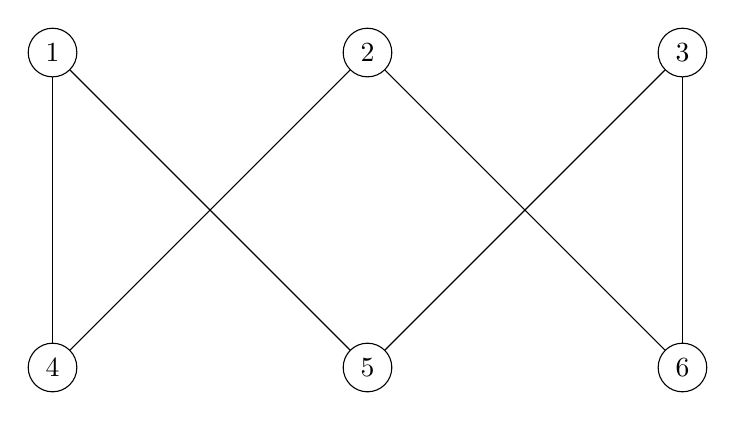
\begin{tikzpicture}[node distance={40mm}, main/.style = {draw, circle}] 
\node[main] (1) {$1$}; 
\node[main] (2) [right of=1] {$2$}; 
\node[main] (3) [right of=2] {$3$}; 
\node[main] (4) [below of=1] {$4$}; 
\node[main] (5) [below of=2] {$5$}; 
\node[main] (6) [below of=3] {$6$}; 

\draw (1) -- (4); 
\draw (1) -- (5); 
\draw (2) -- (4); 
\draw (2) -- (6); 
\draw (3) -- (5); 
\draw (3) -- (6); 
\end{tikzpicture} 
\end{center}
\caption{приклад дводольного графу}
\end{figure}
У даному випадку ми можемо розділити множину вершин на дві:
\begin{center}
$V = U \cup P, P = \{1,2,3\}$ та $U = \{4,5,6\}$.
\end{center}
Немає жодного ребра яке пов'язує вершини множин $P$ із вершинами множини $P$, аналогічно для множини $U$.
\end{example}

\begin{theorem}
В дводольному графі для будь-якого натурального $k$ будь-які вершини однієї долі, де $k$ не перевищує числа вершин доль, пов'язані принаймні з $k$ різними вершинами іншої долі тоді і лише тоді, коли граф розбивається на пари першою часткою.
\end{theorem}

\section{Постановка задачі}

\begin{theorem}
Довести {\bf Теорему 1} у тому вигляді, у якому вона описана, зважаючи лише на те що об'єкт $M$ у твердженні теореми тепер може мати мультимножинну природу \cite{my_article:2021}.
\end{theorem}

\begin{proof}
Використаємо підхід, який базується на {\bf Теоремі 2}. У даному доведенні буде описуватись один з можливих підходів рішення та доведення {\bf даної теореми} через навантаження ребер двочасткового графу певними коефіцієнтами.
У моїй бакалаврській роботі було розглянуто такі випадки: 
\begin{center}
$A = \{z^m,x^m\}, B = \{w_0^{2}, w_1,...,w_n\}$
\end{center}

Як вже було доведено раніше у {\bf Теоремі 1} для звичайного типу множин завжди існує паросполучення при додаванні до сімейства невкладених множин розміру $n$ одного елемента для того, щоб утворити сімейство невкладених множин якому належать множини розміру $n+1$. Для звичайного випадка теореми це і доводить, що максимально можливий розмір такого сімейства ${C_n}^{[n/2]}$. Для випадка коли множина має мультимножинну природу використати {\bf Теорему 1} у тому вигляді як описано вище неможливо.

\begin{example}

Розглянемо множину $ A = \{2,3,4\} $, збудуємо наповнення одноелементного сімейства невключних одна в одну множин, які добудуємо до двоелементного сімейства:
\begin{figure}
\begin{center}
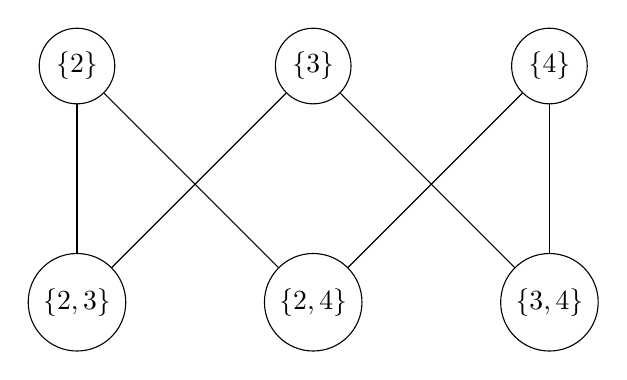
\begin{tikzpicture}[node distance={30mm}, main/.style = {draw, circle}] 
\node[main] (1) {$\{2\}$}; 
\node[main] (2) [right of=1] {$\{3\}$}; 
\node[main] (3) [right of=2] {$\{4\}$}; 
\node[main] (4) [below of=1] {$\{2,3\}$}; 
\node[main] (5) [below of=2] {$\{2,4\}$}; 
\node[main] (6) [below of=3] {$\{3,4\}$}; 

\draw (1) -- (4); 
\draw (1) -- (5); 
\draw (2) -- (4); 
\draw (2) -- (6); 
\draw (3) -- (5); 
\draw (3) -- (6); 
\end{tikzpicture} 
\end{center}
\caption{граф з вагами, для мультимножини $ A = \{2,3,4\}$}
\end{figure}
\end{example}

Ідея полягає в тому, щоб перенести підхід паросполучення використовуючи вагові коефіцієнти.
Як можна бачити з малюнка:
\begin{center}
$ \underline{deg} = t $
\\
$ \overline{deg} = n - t $
\end{center}
Але це можливо лише для випадку коли відповідні ребра навантажені вагами. Нижче буде розглянуто декілька прикладів для розуміння повної картини.
\end{proof}


\begin{example}

Розглянемо множину $ A = \{2^3,3^2\} $, збудуємо наповнення двоелементного сімейства невключних одна в одну множин, які добудуємо до триелементного сімейства:
\begin{figure}
\begin{center}
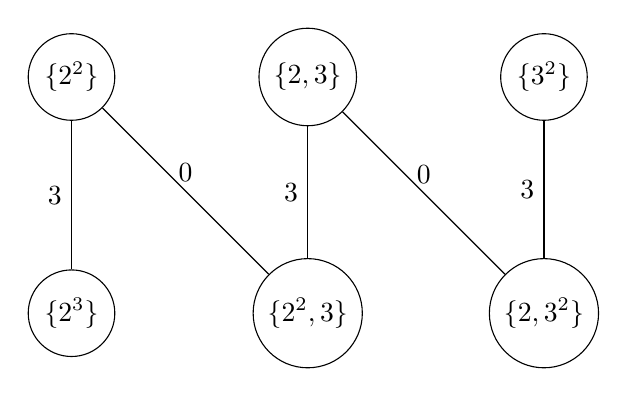
\begin{tikzpicture}[node distance={30mm}, main/.style = {draw, circle}] 
\node[main] (1) {$\{2^2\}$}; 
\node[main] (2) [right of=1] {$\{2,3\}$}; 
\node[main] (3) [right of=2] {$\{3^2\}$}; 
\node[main] (4) [below of=1] {$\{2^3\}$}; 
\node[main] (5) [below of=2] {$\{2^2,3\}$}; 
\node[main] (6) [below of=3] {$\{2,3^2\}$}; 

\draw (1) -- node[left] {3} (4); 
\draw (1) -- node[above] {0} (5); 
\draw (2) -- node[left] {3} (5); 
\draw (2) -- node[above] {0} (6); 
\draw (3) -- node[left] {3} (6); 
\end{tikzpicture} 
\end{center}
\caption{граф з вагами, для мультимножини $ A = \{2,3,4\}$}
\end{figure}
\end{example}

\newpage

\begin{example}
Розглянемо множину $ A = \{2^3,3^3\} $, також збудуємо наповнення двоелементного сімейства невключних одна в одну множин, які добудуємо до триелементного сімейства:
\begin{figure}
\begin{center}
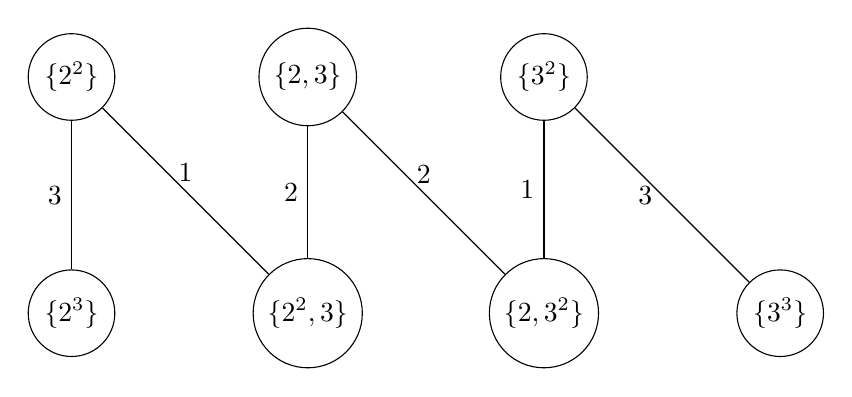
\begin{tikzpicture}[node distance={30mm}, main/.style = {draw, circle}] 
\node[main] (1) {$\{2^2\}$}; 
\node[main] (2) [right of=1] {$\{2,3\}$}; 
\node[main] (3) [right of=2] {$\{3^2\}$}; 
\node[main] (4) [below of=1] {$\{2^3\}$}; 
\node[main] (5) [below of=2] {$\{2^2,3\}$};
\node[main] (6) [below of=3] {$\{2,3^2\}$}; 
\node[main] (7) [right of=6] {$\{3^3\}$}; 

\draw (1) -- node[left]  {3} (4); 
\draw (1) -- node[above] {1} (5); 
\draw (2) -- node[left]  {2} (5); 
\draw (2) -- node[above] {2} (6); 
\draw (3) -- node[left]  {1} (6); 
\draw (3) -- node[left]  {3} (7); 
\end{tikzpicture} 
\end{center}
\caption{граф з вагами, для мультимножини $  A = \{2^3,3^3\} $}
\end{figure}
\end{example}

Тобто обрахунок ведеться за допомогою формул:
\begin{center}
$ \underline{deg} = t $
\\
$ \overline{deg} = n - t $
\end{center}
$n$ - мультипотужність множини на основі якої будується сімейство невкладених одна в одну множин
\\
$t$ - мультипотужність множини яка належить сімейству невкладених одна в одну множин (для $\underline{deg}
$, $t$ - це потужність множини яка належить нижній долі, для  $\overline{deg}$, $t$ - це потужність множини яка належить верхній долі)

Тобто для {\bf Прикладу 4}:
\begin{center}
$ \underline{deg} = 3 $ - оскільки $ |\{2^3\}| = |\{2^2,3\}| = |\{2,3^2\}| $
\\
$ \overline{deg} = |A| - 2 = 3 $ - оскільки $ |A| = 5, |\{2^2\}| = |\{2,3\}| = |\{3^2\}| = 2 $
\end{center}
Далі складається система лінійних рівнянь:

\begin{figure}
\begin{center}
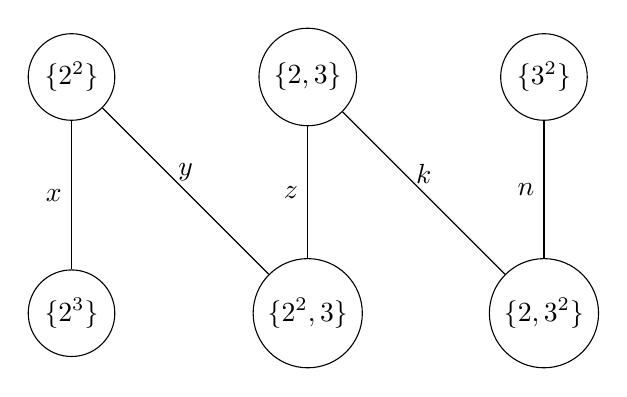
\begin{tikzpicture}[node distance={30mm}, main/.style = {draw, circle}] 
\node[main] (1) {$\{2^2\}$}; 
\node[main] (2) [right of=1] {$\{2,3\}$}; 
\node[main] (3) [right of=2] {$\{3^2\}$}; 
\node[main] (4) [below of=1] {$\{2^3\}$}; 
\node[main] (5) [below of=2] {$\{2^2,3\}$}; 
\node[main] (6) [below of=3] {$\{2,3^2\}$}; 

\draw (1) -- node[left] {$x$} (4); 
\draw (1) -- node[above] {$y$} (5); 
\draw (2) -- node[left] {$z$} (5); 
\draw (2) -- node[above] {$k$} (6); 
\draw (3) -- node[left] {$n$} (6); 
\end{tikzpicture} 
\end{center}
\caption{граф з вагами, для мультимножини $  A = \{2^3,3^3\} $}
\end{figure}
\begin{center}
$\left \{
\begin{tabular}{ccc}
x = 3 \\
x + y = 3 \\ 
y + z = 3 \\
z + k = 3 \\ 
k + n = 3 
  \end{tabular}
    \Rightarrow 
$
$
\left \{
  \begin{tabular}{ccc}
x = 3 \\
y = 0 \\ 
z = 3 \\
k = 0 \\ 
n = 3 
  \end{tabular}
$
\end{center}

Для {\bf Прикладу 5}:
\begin{center}
$ \underline{deg} = 3 $ - оскільки $ |\{2^3\}| = |\{2^2,3\}| = |\{3^3\}| $
\\
$ \overline{deg} = |A| - 2 = 4 $ - оскільки $ |A| = 6, |\{2^2\}| = |\{2,3\}| = |\{3^2\}| = 2 $
\end{center}
Далі складається система лінійних рівнянь:
\begin{figure}
\begin{center}
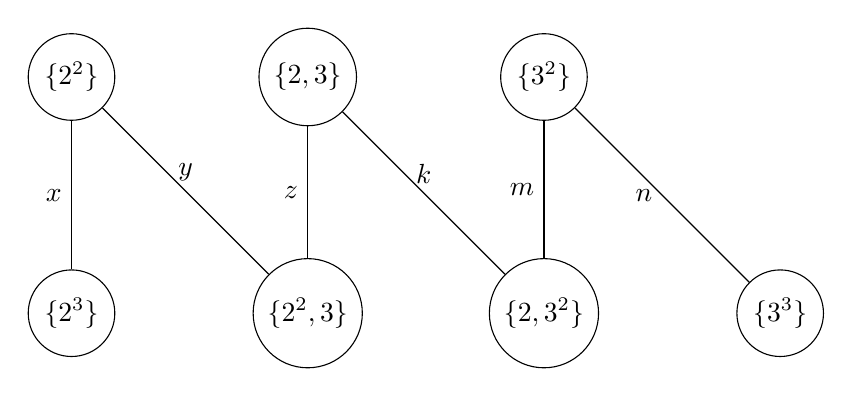
\begin{tikzpicture}[node distance={30mm}, main/.style = {draw, circle}] 
\node[main] (1) {$\{2^2\}$}; 
\node[main] (2) [right of=1] {$\{2,3\}$}; 
\node[main] (3) [right of=2] {$\{3^2\}$}; 
\node[main] (4) [below of=1] {$\{2^3\}$}; 
\node[main] (5) [below of=2] {$\{2^2,3\}$};
\node[main] (6) [below of=3] {$\{2,3^2\}$}; 
\node[main] (7) [right of=6] {$\{3^3\}$}; 

\draw (1) -- node[left]  {$x$} (4); 
\draw (1) -- node[above] {$y$} (5); 
\draw (2) -- node[left]  {$z$} (5); 
\draw (2) -- node[above] {$k$} (6); 
\draw (3) -- node[left]  {$m$} (6); 
\draw (3) -- node[left]  {$n$} (7); 
\end{tikzpicture} 
\end{center}
\caption{граф з вагами, для мультимножини $  A = \{2^3,3^3\} $}
\end{figure}

\begin{center}
$\left \{
\begin{tabular}{ccc}
x = 3 \\
x + y = 4 \\ 
y + z = 3 \\
z + k = 4 \\ 
k + m = 3 \\ 
n = 3 
  \end{tabular}
    \Rightarrow 
$
$
\left \{
  \begin{tabular}{ccc}
x = 3 \\
y = 1 \\ 
z = 2 \\
k = 2 \\ 
m = 1 \\
n = 3
 
  \end{tabular}
$
\end{center}

Таким способом у бакалаврській роботі було доведено випадки $A = \{z^m,x^m\}, B = \{w_0^{2}, w_1,...,w_n\}$. У наступному розділі буде розглянуто декілька інших часткових випадків, для яких буде доведено {\bf Теорему 1}, та будуть записані явні формули обрахунку вагів для графу. За допомогою цих формул можна переконатись, що паросполучення існує і побудувати його явно. Таким чином доводиться для множин мультимножинної природи справедливість {\bf Теореми 1}. Прикладе застосування математичних об'єктів, які задовольняють умови теореми буде описано у роздулах пізніше.

\section*{Висновки до розділу 1}
\addcontentsline{toc}{chapter}{Висновки до розділу 1}

	Розглянуто необхідний математичний апарат, необхідний для розв'язку поставленої задачі. Сформовано твердження ускладненого випадку теореми. Запропоновано підхід для доведення та показано матеріали, які вже були представдені у мохй бакалаврській роботі.
	
	
\newpage

\chapter{Часткові випадки теореми}
\section{Частковий випадок $A = \{a^m, b, c\}$}

Почнемо розглядати новий випадок мультимножини виду $A = \{a^m, b, c\}$, яка задовольняє умови {\bf Теореми 1} \cite{my_article:2021}. На елемент $a^m$ накладаються деякі обмеження, а саме: $m \geq 3 $, оскільки при $ m = 1 $ висхідна множина втрачає мультимножинні властивості, щодо випадку коли  $ m = 2 $, то цей випадок вже був розглянутий у бакалаврській роботі, та включається у випадок $B = \{w_0^{2}, w_1,...,w_n\}$. Почнемо з частинних випадків коли  $ m $ набуває конкретних значень, щоб побачити закономірності у зажуванні дводольного графу та формули за допомогою яких будуть обраховуватись ваги \cite{my_article:2021}.

\begin{example}

Розглянемо множи ну $ A = \{a^3, b, c\} $, збудуємо наповнення двоелементного сімейства невключних одна в одну множин, які добудуємо до триелементного сімейства:
\begin{figure}
\begin{center}
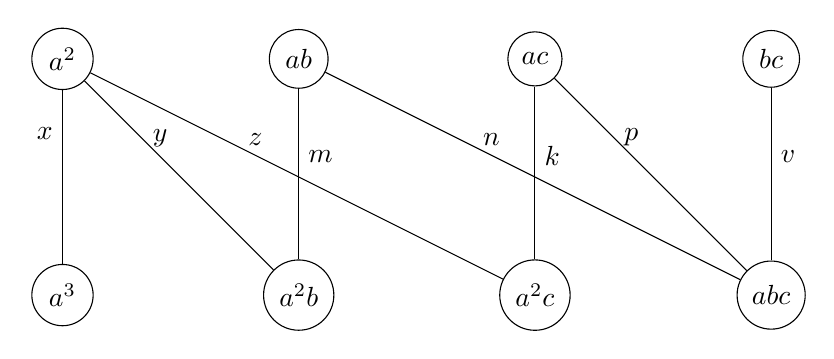
\begin{tikzpicture}[node distance={30mm}, main/.style = {draw, circle}] 
\node[main] (1) {$a^2$}; 
\node[main] (2) [right of=1] {$ab$}; 
\node[main] (3) [right of=2] {$ac$}; 
\node[main] (4) [right of=3] {$bc$}; 
\node[main] (5) [below of=1] {$a^3$}; 
\node[main] (6) [below of=2] {$a^2b$}; 
\node[main] (7) [below of=3] {$a^2c$}; 
\node[main] (8) [below of=4] {$abc$}; 

\draw (1) -- node[pos=0.25, left] {$x$} (5); 
\draw (1) -- node[pos=0.4, above] {$y$} (6); 
\draw (1) -- node[pos=0.4, above] {$z$} (7); 

\draw (2) -- node[pos=0.4, right] {$m$}(6); 
\draw (2) -- node[pos=0.4, above] {$n$}(8); 

\draw (3) -- node[pos=0.4, right] {$k$}(7); 
\draw (3) -- node[pos=0.4, above] {$p$}(8); 
\draw (4) -- node[pos=0.4, right] {$v$}(8); 
\end{tikzpicture} 
\end{center}
\caption{граф з вагами, для мультимножини $ A = \{a^3, b, c\}$}
\end{figure}

\end{example}

Так само, як і у випадках раніше підрахуємо значення вагів за формулою:
\begin{center}
$ \underline{deg} = 3 $ - оскільки $ |\{a^3\}| = |\{a^2,b\}| = |\{a^2,c\}| = |\{a,b,c\}| $
\\
$ \overline{deg} = |A| - 2 = 3 $ - оскільки $ |A| = 5, |\{a^2\}| = |\{a,b\}| = |\{b,c\}| =  |\{a,c\}| = 2 $
\end{center}

\begin{center}
$\left \{
\begin{tabular}{ccc}
x = 3 \\
x + y + z = 3 \\ 
m + y = 3 \\
m + n = 3 \\
z + k = 3 \\
k + p = 3 \\
n + p + v = 3 \\ 
v = 3 
  \end{tabular}
    \Rightarrow 
$
$
\left \{
  \begin{tabular}{ccc}
x = 3 \\
y = 0 \\ 
z = 0 \\
m = 3 \\ 
n = 0 \\
k = 3 \\
p = 0 \\
v = 3
 
  \end{tabular}
$
\end{center}

Для випадку коли  вага ребра дорівнює $ 0 $, виключаємо таке ребро із графу, тобто отримали повне паросполучення:
\begin{figure}
\begin{center}
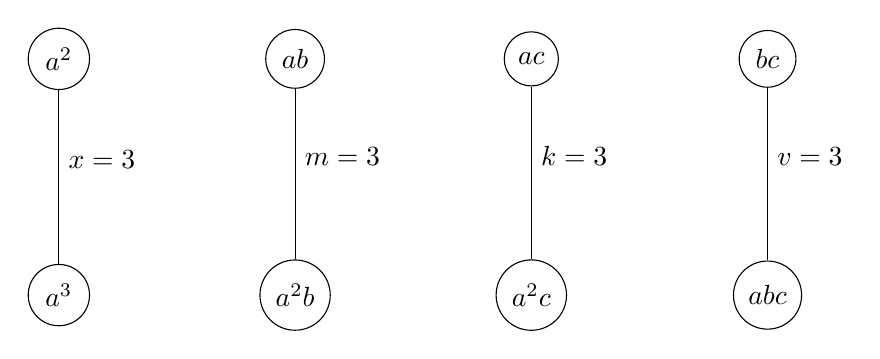
\begin{tikzpicture}[node distance={30mm}, main/.style = {draw, circle}] 
\node[main] (1) {$a^2$}; 
\node[main] (2) [right of=1] {$ab$}; 
\node[main] (3) [right of=2] {$ac$}; 
\node[main] (4) [right of=3] {$bc$}; 
\node[main] (5) [below of=1] {$a^3$}; 
\node[main] (6) [below of=2] {$a^2b$}; 
\node[main] (7) [below of=3] {$a^2c$}; 
\node[main] (8) [below of=4] {$abc$}; 

\draw (1) -- node[pos=0.4,right] {$x = 3$}(5); 
\draw (2) -- node[pos=0.4, right] {$m = 3$}(6); 
\draw (3) -- node[pos=0.4, right] {$k = 3$}(7); 
\draw (4) -- node[pos=0.4, right] {$v = 3$}(8); 
\end{tikzpicture} 
\end{center}
\caption{граф з вагами, для мультимножини $ A = \{a^3, b, c\}$}
\end{figure}


Розглянемо множину $ A = \{a^4, b, c\} $, так само збудуємо наповнення двоелементного сімейства невключних одна в одну множин, які добудуємо до триелементного сімейства:
\begin{figure}
\begin{center}
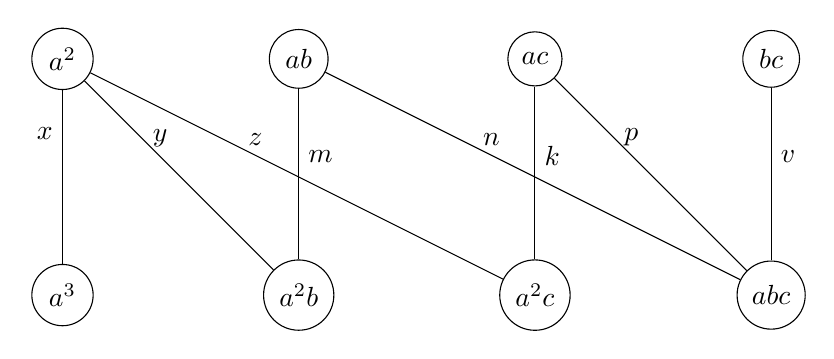
\begin{tikzpicture}[node distance={30mm}, main/.style = {draw, circle}] 
\node[main] (1) {$a^2$}; 
\node[main] (2) [right of=1] {$ab$}; 
\node[main] (3) [right of=2] {$ac$}; 
\node[main] (4) [right of=3] {$bc$}; 
\node[main] (5) [below of=1] {$a^3$}; 
\node[main] (6) [below of=2] {$a^2b$}; 
\node[main] (7) [below of=3] {$a^2c$}; 
\node[main] (8) [below of=4] {$abc$}; 

\draw (1) -- node[pos=0.25, left] {$x$} (5); 
\draw (1) -- node[pos=0.4, above] {$y$} (6); 
\draw (1) -- node[pos=0.4, above] {$z$} (7); 

\draw (2) -- node[pos=0.4, right] {$m$}(6); 
\draw (2) -- node[pos=0.4, above] {$n$}(8); 

\draw (3) -- node[pos=0.4, right] {$k$}(7); 
\draw (3) -- node[pos=0.4, above] {$p$}(8); 
\draw (4) -- node[pos=0.4, right] {$v$}(8); 
\end{tikzpicture} 
\end{center}
\caption{граф з вагами, для мультимножини  $ A = \{a^4, b, c\} $}
\end{figure}

Так само як для попереднього випадку:
\begin{center}
$ \underline{deg} = 3 $ - оскільки $ |\{a^3\}| = |\{a^2,b\}| = |\{a^2,c\}| = |\{a,b,c\}| $
\\
$ \overline{deg} = |A| - 2 = 3 $ - оскільки $ |A| = 5, |\{a^2\}| = |\{a,b\}| = |\{b,c\}| =  |\{a,c\}| = 2 $
\end{center}

\begin{center}
$\left \{
\begin{tabular}{ccc}
x = 3 \\
x + y + z = 3 \\ 
m + y = 3 \\
m + n = 3 \\
z + k = 3 \\
k + p = 3 \\
n + p + v = 3 \\ 
v = 3 
  \end{tabular}
    \Rightarrow 
$
$
\left \{
  \begin{tabular}{ccc}
x = 3 \\
y = 0 \\ 
z = 0 \\
m = 3 \\ 
n = 0 \\
k = 3 \\
p = 0 \\
v = 3
 
  \end{tabular}
$
\end{center}

Для випадку коли  вага ребра дорівнює $ 0 $, ми виключаємо таке ребро із графу, тобто ми отримали повне паросполучення:
\begin{figure}
\begin{center}
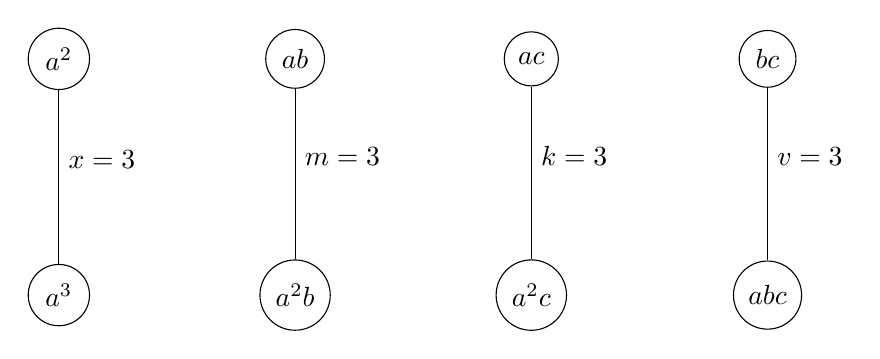
\begin{tikzpicture}[node distance={30mm}, main/.style = {draw, circle}] 
\node[main] (1) {$a^2$}; 
\node[main] (2) [right of=1] {$ab$}; 
\node[main] (3) [right of=2] {$ac$}; 
\node[main] (4) [right of=3] {$bc$}; 
\node[main] (5) [below of=1] {$a^3$}; 
\node[main] (6) [below of=2] {$a^2b$}; 
\node[main] (7) [below of=3] {$a^2c$}; 
\node[main] (8) [below of=4] {$abc$}; 

\draw (1) -- node[pos=0.4,right] {$x = 3$}(5); 
\draw (2) -- node[pos=0.4, right] {$m = 3$}(6); 
\draw (3) -- node[pos=0.4, right] {$k = 3$}(7); 
\draw (4) -- node[pos=0.4, right] {$v = 3$}(8); 
\end{tikzpicture} 
\end{center}
\caption{граф з вагами, для мультимножини  $ A = \{a^4, b, c\} $}
\end{figure}

Ми отримали точно такий же граф, як і у попередньому випадку, навіть з такими же вагами. Давайте спробуємо узагальнити підхід для випадку коли $ A = \{a^m, b, c\} $. Я буду спиратись на твердження, яке було доведене у моїй бакалаврській роботі:

\begin{center}
$ C_n^{k} \leq C_n^{k+1} $, для випадку коли $ k < [n/2]$, де $n$ - це кількість елементів висхідної множини, $k$ - потужність підмножини.
\end{center}

Отже, за припущенням найбільше сімейство мультипідможин, які невключаються одна в одну, тобто максимальна потужність такого сімейства набувається коли потужність кожної окремої множини дорівнює $ [n/2] $. $|A| = m + 2$, тоді побудуємо перехід від $ [(m+2)/2 - 1]$ елементних підмножин до $ [(m+2)/2]$:

\begin{example}


Розглянемо множину $ A = \{a^m, b, c\} $:
\begin{figure}
\begin{center}
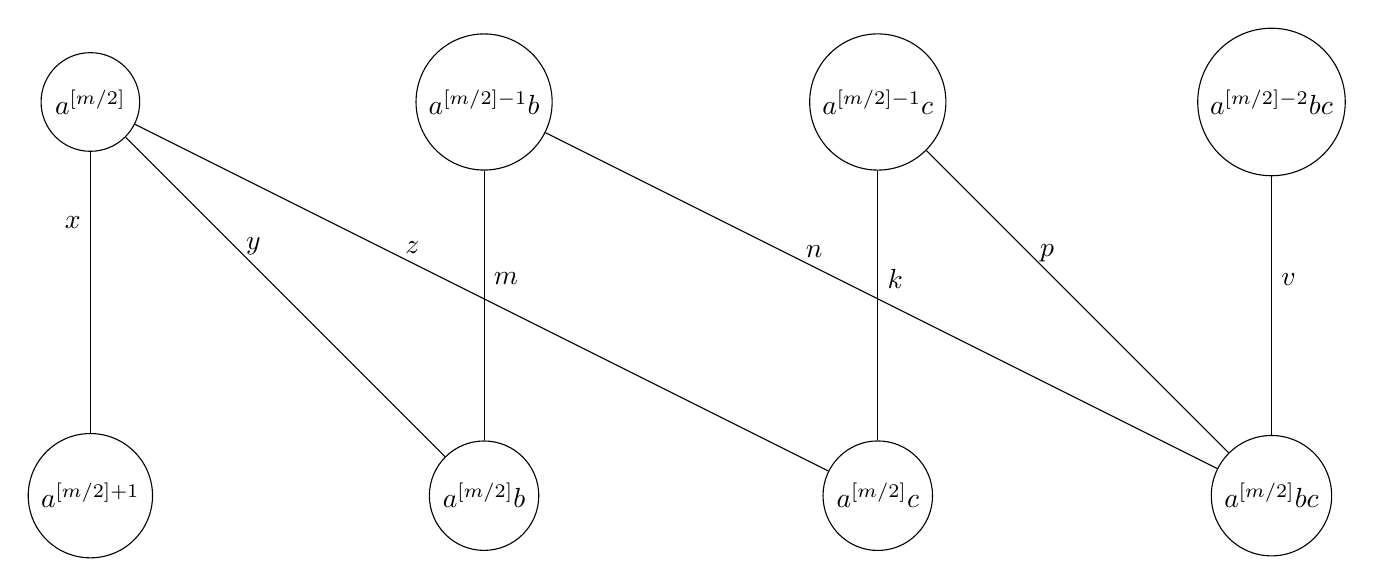
\begin{tikzpicture}[node distance={50mm}, main/.style = {draw, circle}] 
\node[main] (1) {$a^{[m/2]}$}; 
\node[main] (2) [right of=1] {$a^{[m/2] - 1}b$}; 
\node[main] (3) [right of=2] {$a^{[m/2] - 1}c$}; 
\node[main] (4) [right of=3] {$a^{[m/2] - 2}bc$}; 
\node[main] (5) [below of=1] {$a^{[m/2] + 1}$}; 
\node[main] (6) [below of=2] {$a^{[m/2]}b$}; 
\node[main] (7) [below of=3] {$a^{[m/2]}c$}; 
\node[main] (8) [below of=4] {$a^{[m/2]}bc$}; 

\draw (1) -- node[pos=0.25, left] {$x$} (5); 
\draw (1) -- node[pos=0.4, above] {$y$} (6); 
\draw (1) -- node[pos=0.4, above] {$z$} (7); 

\draw (2) -- node[pos=0.4, right] {$m$}(6); 
\draw (2) -- node[pos=0.4, above] {$n$}(8); 

\draw (3) -- node[pos=0.4, right] {$k$}(7); 
\draw (3) -- node[pos=0.4, above] {$p$}(8); 
\draw (4) -- node[pos=0.4, right] {$v$}(8); 
\end{tikzpicture} 
\end{center}
\caption{граф з вагами, для мультимножини  $ A = \{a^m, b, c\} $}
\end{figure}
\end{example}

Так само як для попереднього випадку:
\begin{center}
$ \underline{deg} = [m/2] + 1 $
\\
$ \overline{deg} = |A| - [m/2] = m + 2 - [m/2] $
\end{center}

\begin{center}
$\left \{
\begin{tabular}{ccc}
x = [m/2] + 1 \\
x + y + z = m + 2 - [m/2] \\ 
m + y = [m/2] + 1  \\
m + n = m + 2 - [m/2] \\
z + k = [m/2] + 1 \\
k + p = m + 2 - [m/2]  \\
n + p + v = [m/2] + 1 \\ 
v = [m/2] + 1 
  \end{tabular}
$
\end{center}

Для випадку коли $ A = \{a^m, b, c\} $ ми отримали явні формули підрахунку вагів ребер графу, для заданого  $ m $ треба розв'язати систему лінійних рівнянь методом Гауса, та отримати ваги, які увантажать граф. 
\\
Якщо зробити перевірку, та підставити  $ m = 3 $, той випадок, що вже був розглянутий у {\bf Прикладі 6}:


\begin{center}
$\left \{
\begin{tabular}{ccc}
x = [m/2] + 1 \\
x + y + z = m + 2 - [m/2] \\ 
m + y = [m/2] + 1  \\
m + n = m + 2 - [m/2] \\
z + k = [m/2] + 1 \\
k + p = m + 2 - [m/2]  \\
n + p + v = [m/2] + 1 \\ 
v = [m/2] + 1 
  \end{tabular}
    \Rightarrow 
$
$
\left \{
  \begin{tabular}{ccc}
x = [m/2] + 1 = 2 + 1 = 3\\
x + y + z = m + 2 - [m/2] = 3 \\ 
m + y = [m/2] + 1 = 3 \\
m + n = m + 2 - [m/2] = 3 \\
z + k = [m/2] + 1 = 3\\
k + p = m + 2 - [m/2] = 3  \\
n + p + v = [m/2] + 1 = 3\\ 
v = [m/2] + 1 = 3
 
  \end{tabular}
      \Rightarrow 
$
$
\left \{
  \begin{tabular}{ccc}
x = 3 \\
y = 0 \\ 
z = 0 \\
m = 3 \\ 
n = 0 \\
k = 3 \\
p = 0 \\
v = 3
 
  \end{tabular}
$
\end{center}

\section{Частковий випадок $A = \{a^2, b^2, c\}$}

Розглянемо наступний випадок мультимножини виду $A = \{a^2, b^2, c\}$, яка задовольняє умови {\bf Теореми 1}. На елементи накладаються деякі обмеження, а саме потужність усіх елементів рівна, а один єдиний елемент має потужність одиниця.

\begin{example}

Розглянемо множину $ A = \{a^2, b^2, c\} $, збудуємо наповнення двоелементного сімейства невключних одна в одну множин, які добудуємо до триелементного сімейства:
\begin{figure}
\begin{center}
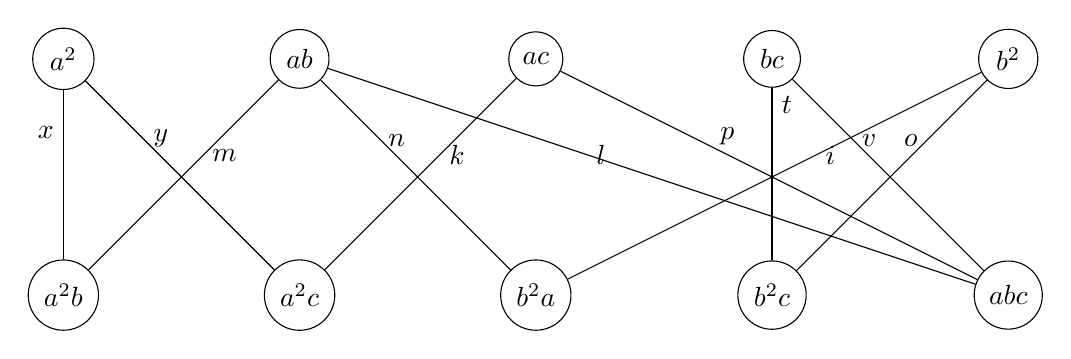
\begin{tikzpicture}[node distance={30mm}, main/.style = {draw, circle}] 
\node[main] (1) {$a^2$}; 
\node[main] (2) [right of=1] {$ab$}; 
\node[main] (3) [right of=2] {$ac$}; 
\node[main] (4) [right of=3] {$bc$}; 
\node[main] (5) [right of=4] {$b^2$}; 

\node[main] (6) [below of=1] {$a^2b$}; 
\node[main] (7) [below of=2] {$a^2c$}; 
\node[main] (8) [below of=3] {$b^2a$}; 
\node[main] (9) [below of=4] {$b^2c$}; 
\node[main] (10) [below of=5] {$abc$}; 

 

\draw (1) -- node[pos=0.25, left] {$x$} (6); 
\draw (1) -- node[pos=0.4, above] {$y$} (7); 

\draw (2) -- node[pos=0.4, right] {$m$}(6); 
\draw (2) -- node[pos=0.4, above] {$n$}(8); 
\draw (2) -- node[pos=0.4, right] {$l$}(10); 


\draw (3) -- node[pos=0.4, right] {$k$}(7); 
\draw (3) -- node[pos=0.4, above] {$p$}(10); 

\draw (4) -- node[pos=0.1, right] {$t$}(9); 
\draw (4) -- node[pos=0.4, above]  {$v$}(10); 

\draw (5) -- node[pos=0.4, right] {$i$}(8); 
\draw (5) -- node[pos=0.4, above] {$o$}(9); 

\end{tikzpicture} 
\end{center}
\caption{граф з вагами, для мультимножини  $ A = \{a^2, b^2, c\} $}
\end{figure}
\end{example}

Так само, як і у випадках раніше підрахуємо значення вагів за формулою:
\begin{center}
$ \underline{deg} = 3 $ - оскільки $ |\{a^2,b\}| = |\{a^2,c\}| = |\{a,b,c\}| = ... $
\\
$ \overline{deg} = |A| - 2 = 3 $, $ |A| = 5, |\{a^2\}| = |\{a,b\}| = |\{b,c\}| =  |\{a,c\}| = ... = 2 $
\end{center}
Розв'яжемо систему лінійних рівнянь за допомогою метода Гауса, запрограмованого на мові програмування Java. У програму треба ввести коефіцієнти при кожній змінній та рівняння по кожній змінній. Нижче записана система лінійних рівнянь та її розв'язок. Як можна побачити усі коефіцієнти невід'ємні та задовольняють умови {\bf Теореми 1}.
\begin{center}
$\left \{
\begin{tabular}{ccc}
x + y = 3 \\
x + m = 3 \\ 
k + y = 3 \\
m + n + l = 3 \\
p + k = 3 \\
n + i = 3 \\
t + v = 3 \\ 
t + b = 3 \\
p + l + v = 3 \\ 
i + l = 3 \\
t + o = 3 \\
  \end{tabular}
\Rightarrow 
$
$\left \{
\begin{tabular}{ccc}
x = 2 \\
y = 1 \\
m = 1 \\ 
p = 1 \\
n = 2 \\
k = 2 \\
v = 2 \\ 
t = 1 \\
l = 0 \\ 
i = 1 \\
o = 2 \\
  \end{tabular}
$
\end{center}

Отже отримали зважений граф при переході від двоелементних мультипідмножин до триелементних мультипідмножин:
\begin{figure}
\begin{center}
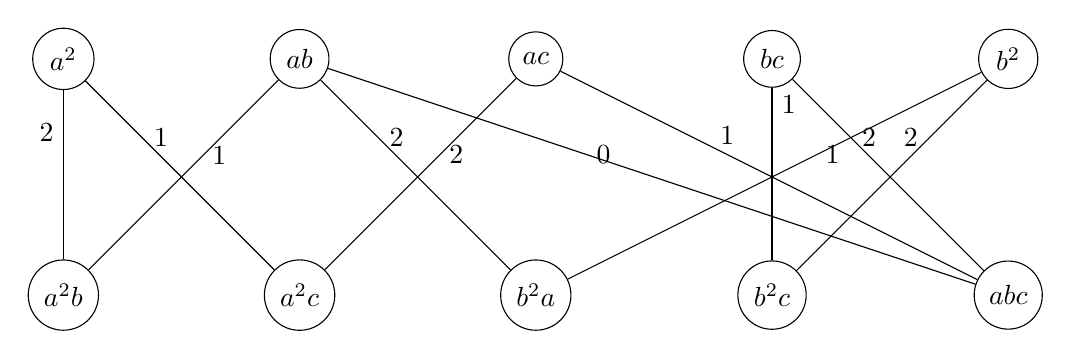
\begin{tikzpicture}[node distance={30mm}, main/.style = {draw, circle}] 
\node[main] (1) {$a^2$}; 
\node[main] (2) [right of=1] {$ab$}; 
\node[main] (3) [right of=2] {$ac$}; 
\node[main] (4) [right of=3] {$bc$}; 
\node[main] (5) [right of=4] {$b^2$}; 

\node[main] (6) [below of=1] {$a^2b$}; 
\node[main] (7) [below of=2] {$a^2c$}; 
\node[main] (8) [below of=3] {$b^2a$}; 
\node[main] (9) [below of=4] {$b^2c$}; 
\node[main] (10) [below of=5] {$abc$}; 

 

\draw (1) -- node[pos=0.25, left] {$2$} (6); 
\draw (1) -- node[pos=0.4, above] {$1$} (7); 

\draw (2) -- node[pos=0.4, right] {$1$}(6); 
\draw (2) -- node[pos=0.4, above] {$2$}(8); 
\draw (2) -- node[pos=0.4, right] {$0$}(10); 


\draw (3) -- node[pos=0.4, right] {$2$}(7); 
\draw (3) -- node[pos=0.4, above] {$1$}(10); 

\draw (4) -- node[pos=0.1, right] {$1$}(9); 
\draw (4) -- node[pos=0.4, above]  {$2$}(10); 

\draw (5) -- node[pos=0.4, right] {$1$}(8); 
\draw (5) -- node[pos=0.4, above] {$2$}(9); 

\end{tikzpicture} 
\end{center}
\caption{граф з вагами, для мультимножини  $ A = \{a^2, b^2, c\} $}
\end{figure}

\section{Частковий випадок $A = \{a^2, b^2, c^2\}$}
Розглянемо наступний випадок мультимножини виду $A = \{a^2, b^2, c^2\}$, яка задовольняє умови {\bf Теореми 1}. На елементи накладаються деякі обмеження, а саме потужність усіх елементів рівна, оскільки при $ m = 1 $ висхідна множина втрачає мультимножинні властивості.

\begin{example}

Розглянемо множину $ A = \{a^2, b^2, c^2\} $, збудуємо наповнення двоелементного сімейства невключних одна в одну множин, які добудуємо до триелементного сімейства:

\begin{figure}
\begin{center}
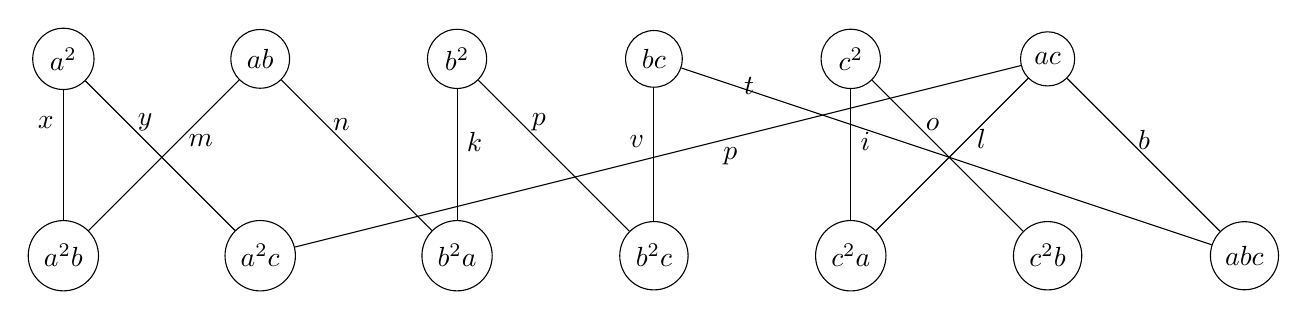
\begin{tikzpicture}[node distance={25mm}, main/.style = {draw, circle}] 
\node[main] (1) {$a^2$}; 
\node[main] (2) [right of=1] {$ab$}; 
\node[main] (3) [right of=2] {$b^2$}; 
\node[main] (4) [right of=3] {$bc$}; 
\node[main] (5) [right of=4] {$c^2$}; 
\node[main] (6) [right of=5] {$ac$}; 

\node[main] (7) [below of=1] {$a^2b$}; 
\node[main] (8) [below of=2] {$a^2c$}; 
\node[main] (9) [below of=3] {$b^2a$}; 
\node[main] (10) [below of=4] {$b^2c$}; 
\node[main] (11) [below of=5] {$c^2a$}; 
\node[main] (12) [below of=6] {$c^2b$};
\node[main] (13) [right of=12] {$abc$}; 
 

\draw (1) -- node[pos=0.25, left] {$x$} (7); 
\draw (1) -- node[pos=0.4, above] {$y$} (8); 

\draw (2) -- node[pos=0.4, right] {$m$}(7); 
\draw (2) -- node[pos=0.4, above] {$n$}(9); 

\draw (3) -- node[pos=0.4, right] {$k$}(9); 
\draw (3) -- node[pos=0.4, above] {$p$}(10); 

\draw (4) -- node[pos=0.4, left] {$v$}(10); 
\draw (4) -- node[pos=0.1, right] {$t$}(13); 

\draw (5) -- node[pos=0.4, right] {$i$}(11); 
\draw (5) -- node[pos=0.4, above] {$o$}(12); 

\draw (6) -- node[pos=0.4, below] {$p$}(8); 
\draw (6) -- node[pos=0.4, right] {$l$}(11); 
\draw (6) -- node[pos=0.4, right] {$b$}(13); 


\end{tikzpicture} 
\end{center}
\caption{граф з вагами, для мультимножини  $ A = \{a^2, b^2, c^2\} $}
\end{figure}
\end{example}

Так само, як і у випадках раніше підрахуємо значення вагів за формулою:
\begin{center}
$ \underline{deg} = 3 $ - оскільки $ |\{a^3\}| = |\{a^2,b\}| = |\{a^2,c\}| = |\{a,b,c\}| = ... $
\\
$ \overline{deg} = |A| - 2 = 4 $, $ |A| = 6, |\{a^2\}| = |\{a,b\}| = |\{b,c\}| =  |\{a,c\}| = ... = 2 $
\end{center}
Розв'яжемо систему лінійних рівнянь за допомогою метода Гауса, запрограмованого на мові програмування Java. У програму треба ввести коефіцієнти при кожній змінній та рівняння по кожній змінній. Нижче записана система лінійних рівнянь та її розв'язок. Як можна побачити усі коефіцієнти невід'ємні та задовольняють умови {\bf Теореми 1}.
\begin{center}
$\left \{
\begin{tabular}{ccc}
x + y = 4 \\
x + m = 3 \\ 
p + y = 3 \\
m + n = 4 \\
p + k = 4 \\
k + p = 4 \\
p + v = 3 \\ 
t + b = 3 \\
b + l + t = 4 \\ 
i + l = 3 \\
i + o = 4 \\
y + t = 3 
  \end{tabular}
\Rightarrow 
$
$\left \{
\begin{tabular}{ccc}
x = 2 \\
y = 2 \\
m = 1 \\ 
p = 1 \\
n = 3 \\
k = 3 \\
v = 2 \\ 
t = 1 \\
b = 2 \\
l = 1 \\ 
i = 2 \\
o = 2 \\
  \end{tabular}
$
\end{center}

Отже отримали зважений граф при переході від двоелементних мультипідмножин до триелементних мультипідмножин:
\begin{figure}
\begin{center}
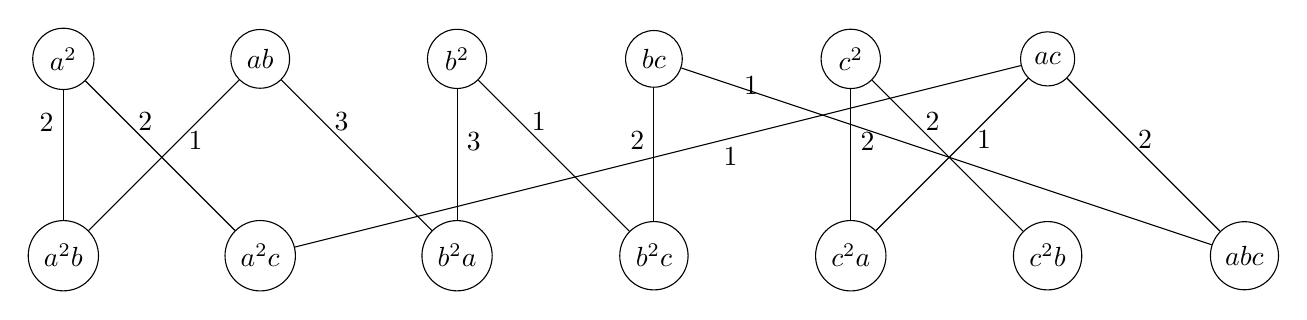
\begin{tikzpicture}[node distance={25mm}, main/.style = {draw, circle}] 
\node[main] (1) {$a^2$}; 
\node[main] (2) [right of=1] {$ab$}; 
\node[main] (3) [right of=2] {$b^2$}; 
\node[main] (4) [right of=3] {$bc$}; 
\node[main] (5) [right of=4] {$c^2$}; 
\node[main] (6) [right of=5] {$ac$}; 

\node[main] (7) [below of=1] {$a^2b$}; 
\node[main] (8) [below of=2] {$a^2c$}; 
\node[main] (9) [below of=3] {$b^2a$}; 
\node[main] (10) [below of=4] {$b^2c$}; 
\node[main] (11) [below of=5] {$c^2a$}; 
\node[main] (12) [below of=6] {$c^2b$};
\node[main] (13) [right of=12] {$abc$}; 
 

\draw (1) -- node[pos=0.25, left] {$2$} (7); 
\draw (1) -- node[pos=0.4, above] {$2$} (8); 

\draw (2) -- node[pos=0.4, right] {$1$}(7); 
\draw (2) -- node[pos=0.4, above] {$3$}(9); 

\draw (3) -- node[pos=0.4, right] {$3$}(9); 
\draw (3) -- node[pos=0.4, above] {$1$}(10); 

\draw (4) -- node[pos=0.4, left] {$2$}(10); 
\draw (4) -- node[pos=0.1, right] {$1$}(13); 

\draw (5) -- node[pos=0.4, right] {$2$}(11); 
\draw (5) -- node[pos=0.4, above] {$2$}(12); 

\draw (6) -- node[pos=0.4, below] {$1$}(8); 
\draw (6) -- node[pos=0.4, right] {$1$}(11); 
\draw (6) -- node[pos=0.4, right] {$2$}(13); 


\end{tikzpicture} 
\end{center}
\caption{граф з вагами, для мультимножини  $ A = \{a^2, b^2, c^2\} $}
\end{figure}


\section{Частковий випадок $A = \{a^3, b, c, d\}$}

Розглянемо наступний випадок мультимножини виду $A = \{a^3, b, c, d\}$, яка задовольняє умови {\bf Теореми 1}. На елементи накладаються деякі обмеження, а саме потужність усіх елементів рівна, а кратність одного елемента три.

\begin{example}

Розглянемо множину $A = \{a^3, b, c, d\}$, збудуємо наповнення триелементного сімейства невключних одна в одну множин, які добудуємо до чотириелементного сімейства:
\begin{figure}
\begin{center}
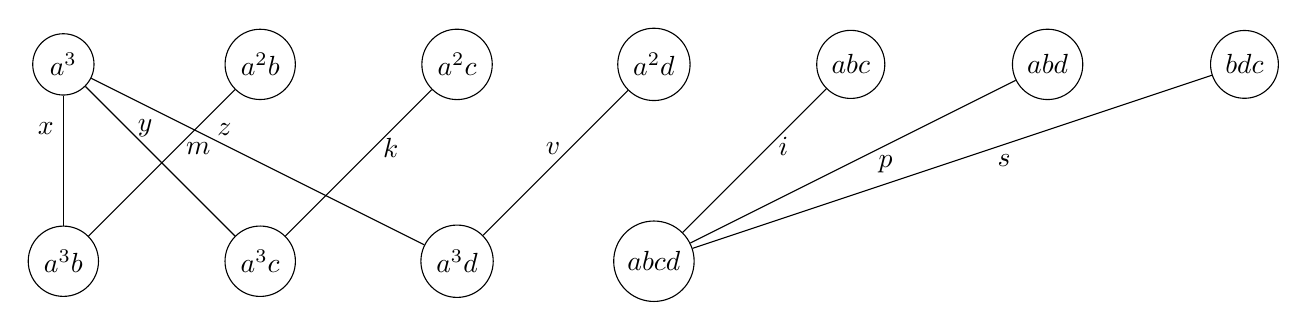
\begin{tikzpicture}[node distance={25mm}, main/.style = {draw, circle}] 
\node[main] (1) {$a^3$}; 
\node[main] (2) [right of=1] {$a^2b$}; 
\node[main] (3) [right of=2] {$a^2c$}; 
\node[main] (4) [right of=3] {$a^2d$}; 
\node[main] (5) [right of=4] {$abc$}; 
\node[main] (6) [right of=5] {$abd$}; 
\node[main] (7) [right of=6] {$bdc$}; 

\node[main] (8) [below of=1] {$a^3b$}; 
\node[main] (9) [below of=2] {$a^3c$}; 
\node[main] (10) [below of=3] {$a^3d$}; 
\node[main] (11) [below of=4] {$abcd$}; 
 

\draw (1) -- node[pos=0.25, left] {$x$} (8); 
\draw (1) -- node[pos=0.4, above] {$y$} (9); 
\draw (1) -- node[pos=0.4, above] {$z$} (10); 


\draw (2) -- node[pos=0.4, right] {$m$}(8); 

\draw (3) -- node[pos=0.4, right] {$k$}(9); 

\draw (4) -- node[pos=0.4, left] {$v$}(10); 

\draw (5) -- node[pos=0.4, right] {$i$}(11); 
\draw (6) -- node[pos=0.4, below] {$p$}(11); 
\draw (7) -- node[pos=0.4, below] {$s$}(11); 


\end{tikzpicture} 
\end{center}
\caption{граф з вагами, для мультимножини  $ A = \{a^3, b, c, d\} $}
\end{figure}
\end{example}

Так само, як і у випадках раніше підрахуємо значення вагів за формулою:
\begin{center}
$ \underline{deg} = 4 $ - оскільки $ |\{a^3b\}| = |\{a^3,c\}| = |\{a^3,d\}| = |\{a,b,c,d\}| = 4 $
\\
$ \overline{deg} = |A| - 3 = 3 $, $ |A| = 6, |\{a^3\}| = |\{a^2,b\}| = ... = 3 $
\end{center}
Розв'яжемо систему лінійних рівнянь за допомогою метода Гауса, запрограмованого на мові програмування Java. У програму треба ввести коефіцієнти при кожній змінній та рівняння по кожній змінній. Нижче записана система лінійних рівнянь та її розв'язок. Як можна побачити усі коефіцієнти невід'ємні та задовольняють умови {\bf Теореми 1}.
\begin{center}
$\left \{
\begin{tabular}{ccc}
x + z = 4 \\
z = 3 \\ 
x + y + m = 3 \\
y + k = 4 \\
v + m = 4 \\
i + p + s = 4 \\
  \end{tabular}
\Rightarrow 
$
$\left \{
\begin{tabular}{ccc}
x = 1 \\
y = 1 \\
k = 3 \\ 
m = 1 \\
v = 3 \\
i = 0 \\
p = 0 \\ 
s = 0 \\
z = 3 \\
  \end{tabular}
$
\end{center}

Отже отримали зважений граф при переході від двоелементних мультипідмножин до триелементних мультипідмножин:
\begin{figure}
\begin{center}
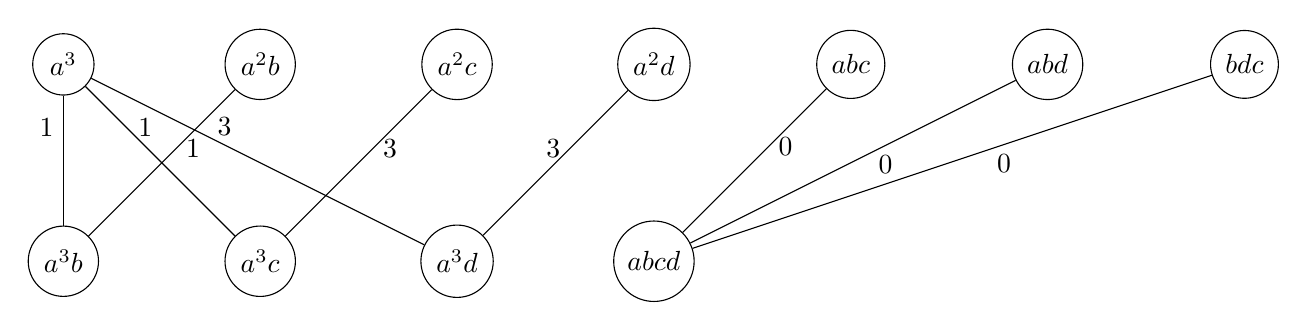
\begin{tikzpicture}[node distance={25mm}, main/.style = {draw, circle}] 
\node[main] (1) {$a^3$}; 
\node[main] (2) [right of=1] {$a^2b$}; 
\node[main] (3) [right of=2] {$a^2c$}; 
\node[main] (4) [right of=3] {$a^2d$}; 
\node[main] (5) [right of=4] {$abc$}; 
\node[main] (6) [right of=5] {$abd$}; 
\node[main] (7) [right of=6] {$bdc$}; 

\node[main] (8) [below of=1] {$a^3b$}; 
\node[main] (9) [below of=2] {$a^3c$}; 
\node[main] (10) [below of=3] {$a^3d$}; 
\node[main] (11) [below of=4] {$abcd$}; 
 

\draw (1) -- node[pos=0.25, left] {$1$} (8); 
\draw (1) -- node[pos=0.4, above] {$1$} (9); 
\draw (1) -- node[pos=0.4, above] {$3$} (10); 


\draw (2) -- node[pos=0.4, right] {$1$}(8); 

\draw (3) -- node[pos=0.4, right] {$3$}(9); 

\draw (4) -- node[pos=0.4, left] {$3$}(10); 

\draw (5) -- node[pos=0.4, right] {$0$}(11); 
\draw (6) -- node[pos=0.4, below] {$0$}(11); 
\draw (7) -- node[pos=0.4, below] {$0$}(11); 


\end{tikzpicture} 
\end{center}
\caption{граф з вагами, для мультимножини  $ A = \{a^3, b, c, d\} $}
\end{figure}


\section{Частковий випадок $A = \{a^2, b^2, c, d\}$}

Розглянемо наступний випадок мультимножини виду $A = \{a^2, b^2, c, d\}$, яка задовольняє умови {\bf Теореми 1}. На елементи накладаються деякі обмеження, а саме потужність усіх елементів рівна, а кратність одного елемента три.

\begin{example}

Розглянемо множину $A = \{a^2, b^2, c, d\}$, збудуємо наповнення триелементного сімейства невключних одна в одну множин, які добудуємо до чотириелементного сімейства:
\begin{figure}
\begin{center}
\begin{tikzpicture}[node distance={30mm}, main/.style = {draw, circle}] 
\node[main] (1) {$a^2b^2$}; 
\node[main] (2) [right of=1] {$a^2cd$}; 
\node[main] (3) [right of=2] {$b^2cd$}; 
\node[main] (4) [right of=3] {$abcd$}; 

\node[main] (5) [below of=1] {$a^2b^2c$}; 
\node[main] (6) [below of=2] {$a^2b^2d$}; 
\node[main] (7) [below of=3] {$a^2bcd$}; 
\node[main] (8) [below of=4] {$b^2acd$}; 
 

\draw (1) -- node[pos=0.25, left] {$x$} (5); 
\draw (1) -- node[pos=0.4, above] {$y$} (6); 

\draw (2) -- node[pos=0.4, right] {$z$}(7); 


\draw (3) -- node[pos=0.4, dbove] {$k$}(8); 

\draw (4) -- node[pos=0.4, left] {$v$}(8);
\draw (4) -- node[pos=0.4, dbove] {$v$}(7); 

\end{tikzpicture} 
\end{center}
\caption{граф з вагами, для мультимножини  $A = \{a^2, b^2, c, d\}$}
\end{figure}
\end{example}

Так само, як і у випадках раніше підрахуємо значення вагів за формулою:
\begin{center}
$ \underline{deg} = 4 $ - оскільки $ |\{a^3b\}| = |\{a^3,c\}| = |\{a^3,d\}| = |\{a,b,c,d\}| = 4 $
\\
$ \overline{deg} = |A| - 3 = 3 $, $ |A| = 6, |\{a^3\}| = |\{a^2,b\}| = ... = 3 $
\end{center}
Розв'яжемо систему лінійних рівнянь за допомогою метода Гауса, запрограмованого на мові програмування Java. У програму треба ввести коефіцієнти при кожній змінній та рівняння по кожній змінній. Нижче записана система лінійних рівнянь та її розв'язок. Як можна побачити усі коефіцієнти невід'ємні та задовольняють умови {\bf Теореми 1}.
\begin{center}
$\left \{
\begin{tabular}{ccc}
x + y = 2 \\
x = 5 \\ 
y = 5 \\
z + k = 5 \\ 
n + m = 5 \\
z = 2 \\
m = 2 \\
  \end{tabular}
\Rightarrow 
$
$\left \{
\begin{tabular}{ccc}
x = 5 \\
y = 5 \\
z = 0 \\ 
k = 5 \\
n = 5 \\
m = 0 \\
  \end{tabular}
$
\end{center}

Отже отримали зважений граф при переході від двоелементних мультипідмножин до триелементних мультипідмножин:

\begin{figure}
\begin{center}
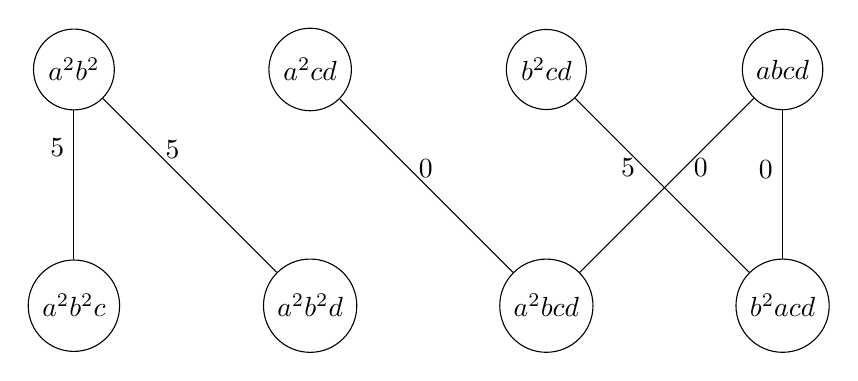
\begin{tikzpicture}[node distance={30mm}, main/.style = {draw, circle}] 
\node[main] (1) {$a^2b^2$}; 
\node[main] (2) [right of=1] {$a^2cd$}; 
\node[main] (3) [right of=2] {$b^2cd$}; 
\node[main] (4) [right of=3] {$abcd$}; 

\node[main] (5) [below of=1] {$a^2b^2c$}; 
\node[main] (6) [below of=2] {$a^2b^2d$}; 
\node[main] (7) [below of=3] {$a^2bcd$}; 
\node[main] (8) [below of=4] {$b^2acd$}; 
 

\draw (1) -- node[pos=0.25, left] {$5$} (5); 
\draw (1) -- node[pos=0.4, above] {$5$} (6); 

\draw (2) -- node[pos=0.4, right] {$0$}(7); 

\draw (3) -- node[pos=0.4, left] {$5$}(8); 

\draw (4) -- node[pos=0.4, left] {$0$}(8);
\draw (4) -- node[pos=0.4, right] {$0$}(7); 

\end{tikzpicture} 
\end{center}
\caption{граф з вагами, для мультимножини  $A = \{a^2, b^2, c, d\}$}
\end{figure}

\section{Частковий випадок $A = \{a^3, b^2, c\}$}

Розглянемо наступний випадок мультимножини виду $A = \{a^3, b^2, c\}$, яка задовольняє умови {\bf Теореми 1}. На елементи накладаються деякі обмеження, а саме потужність елемента $a = 3, b = 2$, а елемент $c$ має потужність одиниця. Для доведення будемо використовувати вже відомий підхід через зважування двочасткового графу.

\begin{example}

Розглянемо множину $ A = \{a^3, b^2, c\} $, збудуємо наповнення 2-елементного сімейства невключних одна в одну множин, які добудуємо до 3-елементного сімейства:
\begin{figure}
\begin{center}
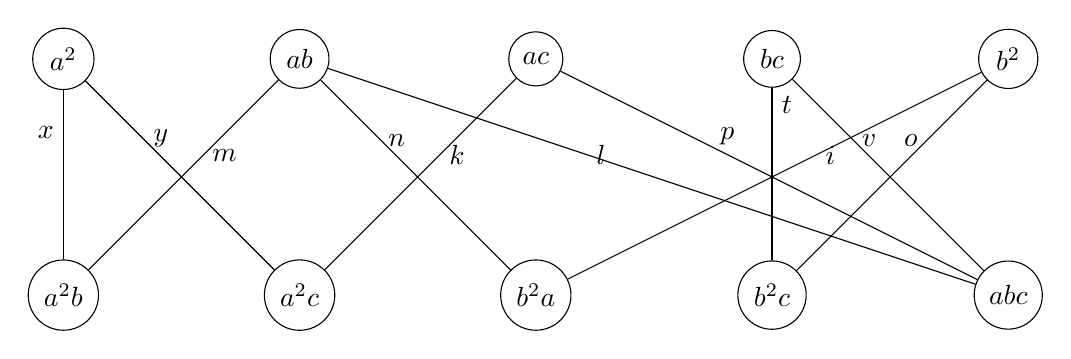
\begin{tikzpicture}[node distance={30mm}, main/.style = {draw, circle}] 
\node[main] (1) {$a^2$}; 
\node[main] (2) [right of=1] {$ab$}; 
\node[main] (3) [right of=2] {$ac$}; 
\node[main] (4) [right of=3] {$bc$}; 
\node[main] (5) [right of=4] {$b^2$}; 

\node[main] (6) [below of=1] {$a^2b$}; 
\node[main] (7) [below of=2] {$a^2c$}; 
\node[main] (8) [below of=3] {$b^2a$}; 
\node[main] (9) [below of=4] {$b^2c$}; 
\node[main] (10) [below of=5] {$abc$}; 

 

\draw (1) -- node[pos=0.25, left] {$x$} (6); 
\draw (1) -- node[pos=0.4, above] {$y$} (7); 

\draw (2) -- node[pos=0.4, right] {$m$}(6); 
\draw (2) -- node[pos=0.4, above] {$n$}(8); 
\draw (2) -- node[pos=0.4, right] {$l$}(10); 


\draw (3) -- node[pos=0.4, right] {$k$}(7); 
\draw (3) -- node[pos=0.4, above] {$p$}(10); 

\draw (4) -- node[pos=0.1, right] {$t$}(9); 
\draw (4) -- node[pos=0.4, above]  {$v$}(10); 

\draw (5) -- node[pos=0.4, right] {$i$}(8); 
\draw (5) -- node[pos=0.4, above] {$o$}(9); 

\end{tikzpicture} 
\end{center}
\caption{граф з вагами, для мультимножини  $A = \{a^3, b^2, c\}$}
\end{figure}
\end{example}

Так само, як і у випадках раніше підрахуємо значення вагів за формулою:
\begin{center}
$ \underline{deg} = 3 $ - оскільки $ |\{a^2,b\}| = |\{a^2,c\}| = |\{a,b,c\}| = ... $
\\
$ \overline{deg} = |A| - 2 = 3 $, $ |A| = 5, |\{a^2\}| = |\{a,b\}| = |\{b,c\}| =  |\{a,c\}| = ... = 2 $
\end{center}
Розв'яжемо систему лінійних рівнянь за допомогою метода Гауса, запрограмованого на мові програмування Java. У програму треба ввести коефіцієнти при кожній змінній та рівняння по кожній змінній. Нижче записана система лінійних рівнянь та її розв'язок. Як можна побачити усі коефіцієнти невід'ємні та задовольняють умови {\bf Теореми 1}. Для розв'язку системи лінійних рівнянь може бути використаний будь-який відомий метод, оскільки у цьому випадку важлива не швидкість розв'язку, а отримані дані. Після отримання вагів для кожного ребра, збудуємо дводольний граф з отриманими вагами для наглядного зображення отриманих результатів. У модулі прикладні застосування буде показано, як можна використовувати підхід зваження у задачах, де ресурси необхідно зрівняти для двох частин системи. 
\begin{center}
$\left \{
\begin{tabular}{ccc}
x + y = 3 \\
x + m = 3 \\ 
k + y = 3 \\
m + n + l = 3 \\
p + k = 3 \\
n + i = 3 \\
t + v = 3 \\ 
t + b = 3 \\
p + l + v = 3 \\ 
i + l = 3 \\
t + o = 3 \\
  \end{tabular}
\Rightarrow 
$
$\left \{
\begin{tabular}{ccc}
x = 2 \\
y = 1 \\
m = 1 \\ 
p = 1 \\
n = 2 \\
k = 2 \\
v = 2 \\ 
t = 1 \\
l = 0 \\ 
i = 1 \\
o = 2 \\
  \end{tabular}
$
\end{center}

Отже отримали зважений граф при переході від двоелементних мультипідмножин до триелементних мультипідмножин:
\begin{figure}
\begin{center}
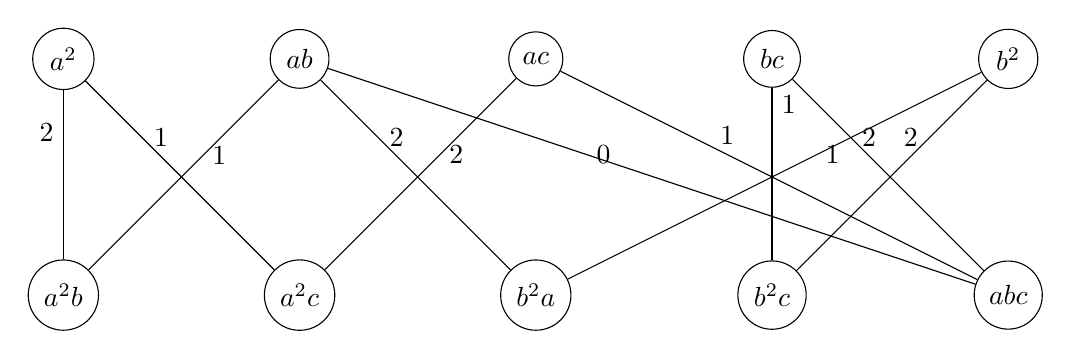
\begin{tikzpicture}[node distance={30mm}, main/.style = {draw, circle}] 
\node[main] (1) {$a^2$}; 
\node[main] (2) [right of=1] {$ab$}; 
\node[main] (3) [right of=2] {$ac$}; 
\node[main] (4) [right of=3] {$bc$}; 
\node[main] (5) [right of=4] {$b^2$}; 

\node[main] (6) [below of=1] {$a^2b$}; 
\node[main] (7) [below of=2] {$a^2c$}; 
\node[main] (8) [below of=3] {$b^2a$}; 
\node[main] (9) [below of=4] {$b^2c$}; 
\node[main] (10) [below of=5] {$abc$}; 

 

\draw (1) -- node[pos=0.25, left] {$2$} (6); 
\draw (1) -- node[pos=0.4, above] {$1$} (7); 

\draw (2) -- node[pos=0.4, right] {$1$}(6); 
\draw (2) -- node[pos=0.4, above] {$2$}(8); 
\draw (2) -- node[pos=0.4, right] {$0$}(10); 


\draw (3) -- node[pos=0.4, right] {$2$}(7); 
\draw (3) -- node[pos=0.4, above] {$1$}(10); 

\draw (4) -- node[pos=0.1, right] {$1$}(9); 
\draw (4) -- node[pos=0.4, above]  {$2$}(10); 

\draw (5) -- node[pos=0.4, right] {$1$}(8); 
\draw (5) -- node[pos=0.4, above] {$2$}(9); 

\end{tikzpicture} 
\end{center}
\caption{граф з вагами, для мультимножини  $A = \{a^3, b^2, c\}$}
\end{figure}


\section{Частковий випадок $A = \{a^4, b^2, c\}$}

Розглянемо наступний випадок мультимножини виду $A = \{a^4, b^2, c\}$, яка задовольняє умови {\bf Теореми 1}. На елементи накладаються деякі обмеження, а саме потужність $a = 4, b = 2, c = 1$. Розглядаючи наповнення сімейств мультипідмножин від двоелементних до триелементних для декількох випадків множини $A = \{a^n, b^2, c\}$  де $n$ - потужність вхождення елементу $a$, варіювання потужності елемента $a$ дає змогу дослідити поводження вагів дводольного графу для того, щоб отримати загальну картину, та отримати змогу узагальнити даний підхід доведення на більшу кількість випадків.

\begin{example}

% Here we'll start 7 examples 
Розглянемо множину $ A = \{a^4, b^2, c\} $, збудуємо наповнення 2-елементного сімейства невключних одна в одну множин, які добудуємо до 3-елементного сімейства:
\begin{figure}
\begin{center}
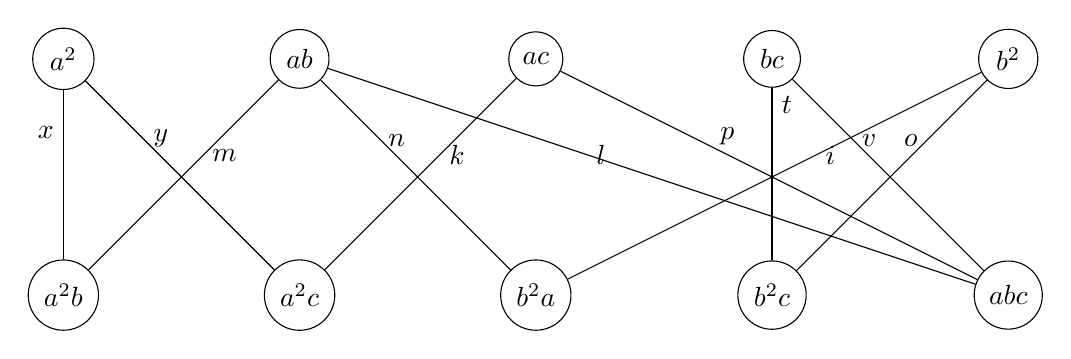
\begin{tikzpicture}[node distance={30mm}, main/.style = {draw, circle}] 
\node[main] (1) {$a^2$}; 
\node[main] (2) [right of=1] {$ab$}; 
\node[main] (3) [right of=2] {$ac$}; 
\node[main] (4) [right of=3] {$bc$}; 
\node[main] (5) [right of=4] {$b^2$}; 

\node[main] (6) [below of=1] {$a^2b$}; 
\node[main] (7) [below of=2] {$a^2c$}; 
\node[main] (8) [below of=3] {$b^2a$}; 
\node[main] (9) [below of=4] {$b^2c$}; 
\node[main] (10) [below of=5] {$abc$}; 

 

\draw (1) -- node[pos=0.25, left] {$x$} (6); 
\draw (1) -- node[pos=0.4, above] {$y$} (7); 

\draw (2) -- node[pos=0.4, right] {$m$}(6); 
\draw (2) -- node[pos=0.4, above] {$n$}(8); 
\draw (2) -- node[pos=0.4, right] {$l$}(10); 


\draw (3) -- node[pos=0.4, right] {$k$}(7); 
\draw (3) -- node[pos=0.4, above] {$p$}(10); 

\draw (4) -- node[pos=0.1, right] {$t$}(9); 
\draw (4) -- node[pos=0.4, above]  {$v$}(10); 

\draw (5) -- node[pos=0.4, right] {$i$}(8); 
\draw (5) -- node[pos=0.4, above] {$o$}(9); 

\end{tikzpicture} 
\end{center}
\caption{граф з вагами, для мультимножини  $ A = \{a^4, b^2, c\} $}
\end{figure}
\end{example}

Так само, як і у випадках раніше підрахуємо значення вагів за формулою:
\begin{center}
$ \underline{deg} = 3 $ - оскільки $ |\{a^2,b\}| = |\{a^2,c\}| = |\{a,b,c\}| = ... $
\\
$ \overline{deg} = |A| - 2 = 3 $, $ |A| = 5, |\{a^2\}| = |\{a,b\}| = |\{b,c\}| =  |\{a,c\}| = ... = 2 $
\end{center}
Розв'яжемо систему лінійних рівнянь за допомогою метода Гауса, запрограмованого на мові програмування Java. У програму треба ввести коефіцієнти при кожній змінній та рівняння по кожній змінній. Нижче записана система лінійних рівнянь та її розв'язок. Як можна побачити усі коефіцієнти невід'ємні та задовольняють умови {\bf Теореми 1}.
\begin{center}
$\left \{
\begin{tabular}{ccc}
x + y = 3 \\
x + m = 3 \\ 
k + y = 3 \\
m + n + l = 3 \\
p + k = 3 \\
n + i = 3 \\
t + v = 3 \\ 
t + b = 3 \\
p + l + v = 3 \\ 
i + l = 3 \\
t + o = 3 \\
  \end{tabular}
\Rightarrow 
$
$\left \{
\begin{tabular}{ccc}
x = 2 \\
y = 1 \\
m = 1 \\ 
p = 1 \\
n = 2 \\
k = 2 \\
v = 2 \\ 
t = 1 \\
l = 0 \\ 
i = 1 \\
o = 2 \\
  \end{tabular}
$
\end{center}

Отже отримали зважений граф при переході від двоелементних мультипідмножин до триелементних мультипідмножин:
\begin{figure}
\begin{center}
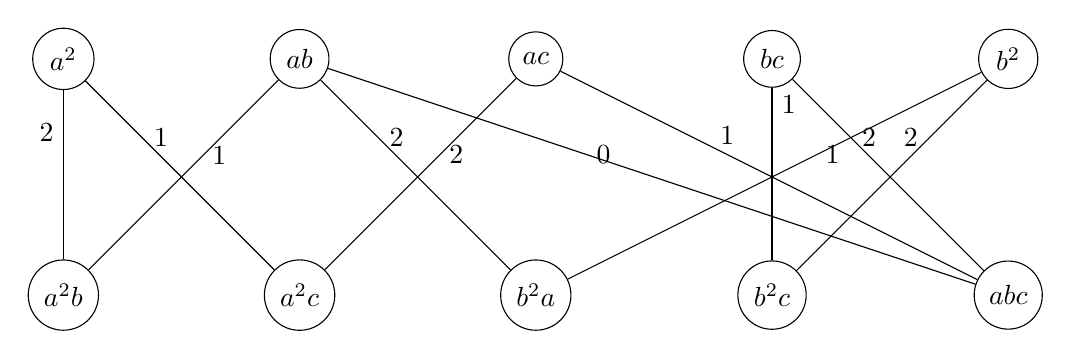
\begin{tikzpicture}[node distance={30mm}, main/.style = {draw, circle}] 
\node[main] (1) {$a^2$}; 
\node[main] (2) [right of=1] {$ab$}; 
\node[main] (3) [right of=2] {$ac$}; 
\node[main] (4) [right of=3] {$bc$}; 
\node[main] (5) [right of=4] {$b^2$}; 

\node[main] (6) [below of=1] {$a^2b$}; 
\node[main] (7) [below of=2] {$a^2c$}; 
\node[main] (8) [below of=3] {$b^2a$}; 
\node[main] (9) [below of=4] {$b^2c$}; 
\node[main] (10) [below of=5] {$abc$}; 

 

\draw (1) -- node[pos=0.25, left] {$2$} (6); 
\draw (1) -- node[pos=0.4, above] {$1$} (7); 

\draw (2) -- node[pos=0.4, right] {$1$}(6); 
\draw (2) -- node[pos=0.4, above] {$2$}(8); 
\draw (2) -- node[pos=0.4, right] {$0$}(10); 


\draw (3) -- node[pos=0.4, right] {$2$}(7); 
\draw (3) -- node[pos=0.4, above] {$1$}(10); 

\draw (4) -- node[pos=0.1, right] {$1$}(9); 
\draw (4) -- node[pos=0.4, above]  {$2$}(10); 

\draw (5) -- node[pos=0.4, right] {$1$}(8); 
\draw (5) -- node[pos=0.4, above] {$2$}(9); 

\end{tikzpicture} 
\end{center}
\caption{граф з вагами, для мультимножини  $ A = \{a^4, b^2, c\} $}
\end{figure}

\section{Частковий випадок $A = \{a^5, b^2, c\}$}

Розглянемо наступний випадок мультимножини виду $A = \{a^5, b^2, c\}$, яка задовольняє умови {\bf Теореми 1}. На елементи накладаються деякі обмеження, а саме потужність усіх елементів рівна, а один єдиний елемент має потужність одиниця. Оскільки вже була розглянута певна кількість випадків теореми, у частині роботи, де буде розгялнуто практичне застосування, є можливість надати явні математичні об'єкти, які можна використовувати у задачі розподілення навантаження. Для "Теорії голосувань" можна отримати верхню оцінку потужності сімейства невкладених одна в одну множин, які мають дуже важливе значення у теорії голосувань.
\begin{example}

Розглянемо множину $ A = \{a^5, b^2, c\} $, збудуємо наповнення двоелементного сімейства невключних одна в одну множин, які добудуємо до триелементного сімейства:
\begin{figure}
\begin{center}
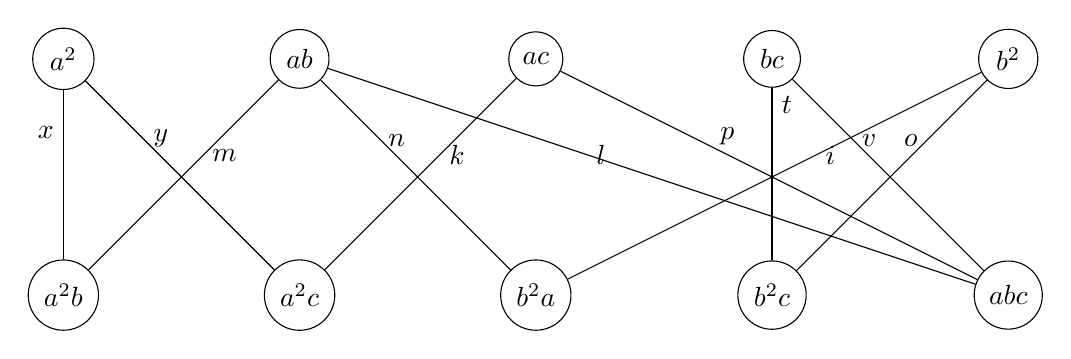
\begin{tikzpicture}[node distance={30mm}, main/.style = {draw, circle}] 
\node[main] (1) {$a^2$}; 
\node[main] (2) [right of=1] {$ab$}; 
\node[main] (3) [right of=2] {$ac$}; 
\node[main] (4) [right of=3] {$bc$}; 
\node[main] (5) [right of=4] {$b^2$}; 

\node[main] (6) [below of=1] {$a^2b$}; 
\node[main] (7) [below of=2] {$a^2c$}; 
\node[main] (8) [below of=3] {$b^2a$}; 
\node[main] (9) [below of=4] {$b^2c$}; 
\node[main] (10) [below of=5] {$abc$}; 

 

\draw (1) -- node[pos=0.25, left] {$x$} (6); 
\draw (1) -- node[pos=0.4, above] {$y$} (7); 

\draw (2) -- node[pos=0.4, right] {$m$}(6); 
\draw (2) -- node[pos=0.4, above] {$n$}(8); 
\draw (2) -- node[pos=0.4, right] {$l$}(10); 


\draw (3) -- node[pos=0.4, right] {$k$}(7); 
\draw (3) -- node[pos=0.4, above] {$p$}(10); 

\draw (4) -- node[pos=0.1, right] {$t$}(9); 
\draw (4) -- node[pos=0.4, above]  {$v$}(10); 

\draw (5) -- node[pos=0.4, right] {$i$}(8); 
\draw (5) -- node[pos=0.4, above] {$o$}(9); 

\end{tikzpicture} 
\end{center}
\caption{граф з вагами, для мультимножини  $ A = \{a^5, b^2, c\} $}
\end{figure}
\end{example}

Так само, як і у випадках раніше підрахуємо значення вагів за формулою:
\begin{center}
$ \underline{deg} = 3 $ - оскільки $ |\{a^2,b\}| = |\{a^2,c\}| = |\{a,b,c\}| = ... $
\\
$ \overline{deg} = |A| - 2 = 3 $, $ |A| = 5, |\{a^2\}| = |\{a,b\}| = |\{b,c\}| =  |\{a,c\}| = ... = 2 $
\end{center}
Розв'яжемо систему лінійних рівнянь за допомогою метода Гауса, запрограмованого на мові програмування Java. У програму треба ввести коефіцієнти при кожній змінній та рівняння по кожній змінній. Нижче записана система лінійних рівнянь та її розв'язок. Як можна побачити усі коефіцієнти невід'ємні та задовольняють умови {\bf Теореми 1}.
\begin{center}
$\left \{
\begin{tabular}{ccc}
x + y = 3 \\
x + m = 3 \\ 
k + y = 3 \\
m + n + l = 3 \\
p + k = 3 \\
n + i = 3 \\
t + v = 3 \\ 
t + b = 3 \\
p + l + v = 3 \\ 
i + l = 3 \\
t + o = 3 \\
  \end{tabular}
\Rightarrow 
$
$\left \{
\begin{tabular}{ccc}
x = 2 \\
y = 1 \\
m = 1 \\ 
p = 1 \\
n = 2 \\
k = 2 \\
v = 2 \\ 
t = 1 \\
l = 0 \\ 
i = 1 \\
o = 2 \\
  \end{tabular}
$
\end{center}

Отже отримали зважений граф при переході від двоелементних мультипідмножин до триелементних мультипідмножин:
\begin{figure}
\begin{center}
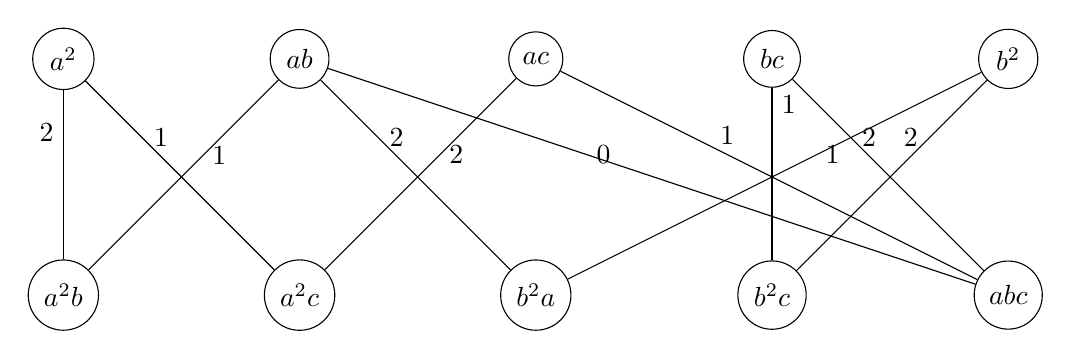
\begin{tikzpicture}[node distance={30mm}, main/.style = {draw, circle}] 
\node[main] (1) {$a^2$}; 
\node[main] (2) [right of=1] {$ab$}; 
\node[main] (3) [right of=2] {$ac$}; 
\node[main] (4) [right of=3] {$bc$}; 
\node[main] (5) [right of=4] {$b^2$}; 

\node[main] (6) [below of=1] {$a^2b$}; 
\node[main] (7) [below of=2] {$a^2c$}; 
\node[main] (8) [below of=3] {$b^2a$}; 
\node[main] (9) [below of=4] {$b^2c$}; 
\node[main] (10) [below of=5] {$abc$}; 

 

\draw (1) -- node[pos=0.25, left] {$2$} (6); 
\draw (1) -- node[pos=0.4, above] {$1$} (7); 

\draw (2) -- node[pos=0.4, right] {$1$}(6); 
\draw (2) -- node[pos=0.4, above] {$2$}(8); 
\draw (2) -- node[pos=0.4, right] {$0$}(10); 


\draw (3) -- node[pos=0.4, right] {$2$}(7); 
\draw (3) -- node[pos=0.4, above] {$1$}(10); 

\draw (4) -- node[pos=0.1, right] {$1$}(9); 
\draw (4) -- node[pos=0.4, above]  {$2$}(10); 

\draw (5) -- node[pos=0.4, right] {$1$}(8); 
\draw (5) -- node[pos=0.4, above] {$2$}(9); 

\end{tikzpicture} 
\end{center}
\caption{граф з вагами, для мультимножини  $ A = \{a^5, b^2, c\} $}
\end{figure}

\section{Частковий випадок $A = \{a^6, b^2, c\}$}

Розглянемо наступний випадок мультимножини виду $A = \{a^6, b^2, c\}$, яка задовольняє умови {\bf Теореми 1}. На елементи накладаються деякі обмеження, а саме потужність усіх елементів рівна, а один єдиний елемент має потужність одиниця. Провівши декілька ітерацій, та отримавши результати для частинних випадків, можна в майбутньому удосконалити підхід, та розробити програму, яка буде самостійно прораховувати ваги для кожного чатинного випадку, тим самим розширюючи кількість частинних випадків, яким задовольняє  {\bf Теорема 1}.

\begin{example}

Розглянемо множину $ A = \{a^6, b^2, c\} $, збудуємо наповнення 2-елементного сімейства невключних одна в одну множин, які добудуємо до 3-елементного сімейства:
\begin{figure}
\begin{center}
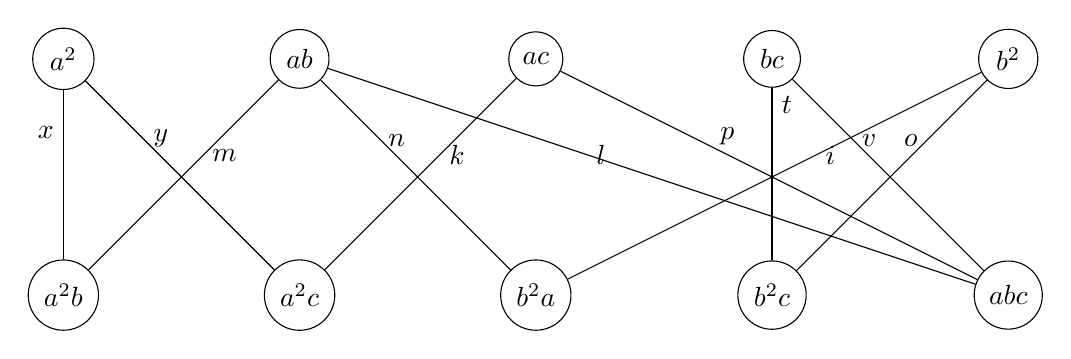
\begin{tikzpicture}[node distance={30mm}, main/.style = {draw, circle}] 
\node[main] (1) {$a^2$}; 
\node[main] (2) [right of=1] {$ab$}; 
\node[main] (3) [right of=2] {$ac$}; 
\node[main] (4) [right of=3] {$bc$}; 
\node[main] (5) [right of=4] {$b^2$}; 

\node[main] (6) [below of=1] {$a^2b$}; 
\node[main] (7) [below of=2] {$a^2c$}; 
\node[main] (8) [below of=3] {$b^2a$}; 
\node[main] (9) [below of=4] {$b^2c$}; 
\node[main] (10) [below of=5] {$abc$}; 

 

\draw (1) -- node[pos=0.25, left] {$x$} (6); 
\draw (1) -- node[pos=0.4, above] {$y$} (7); 

\draw (2) -- node[pos=0.4, right] {$m$}(6); 
\draw (2) -- node[pos=0.4, above] {$n$}(8); 
\draw (2) -- node[pos=0.4, right] {$l$}(10); 


\draw (3) -- node[pos=0.4, right] {$k$}(7); 
\draw (3) -- node[pos=0.4, above] {$p$}(10); 

\draw (4) -- node[pos=0.1, right] {$t$}(9); 
\draw (4) -- node[pos=0.4, above]  {$v$}(10); 

\draw (5) -- node[pos=0.4, right] {$i$}(8); 
\draw (5) -- node[pos=0.4, above] {$o$}(9); 

\end{tikzpicture} 
\end{center}
\caption{граф з вагами, для мультимножини  $ A = \{a^6, b^2, c\} $}
\end{figure}
\end{example}

Так само, як і у випадках раніше підрахуємо значення вагів за формулою:
\begin{center}
$ \underline{deg} = 3 $ - оскільки $ |\{a^2,b\}| = |\{a^2,c\}| = |\{a,b,c\}| = ... $
\\
$ \overline{deg} = |A| - 2 = 3 $, $ |A| = 5, |\{a^2\}| = |\{a,b\}| = |\{b,c\}| =  |\{a,c\}| = ... = 2 $
\end{center}
Нижче записана система лінійних рівнянь та її розв'язок. Як можна побачити усі коефіцієнти невід'ємні та задовольняють умови {\bf Теореми 1}.
\begin{center}
$\left \{
\begin{tabular}{ccc}
x + y = 3 \\
x + m = 3 \\ 
k + y = 3 \\
m + n + l = 3 \\
p + k = 3 \\
n + i = 3 \\
t + v = 3 \\ 
t + b = 3 \\
p + l + v = 3 \\ 
i + l = 3 \\
t + o = 3 \\
  \end{tabular}
\Rightarrow 
$
$\left \{
\begin{tabular}{ccc}
x = 2 \\
y = 1 \\
m = 1 \\ 
p = 1 \\
n = 2 \\
k = 2 \\
v = 2 \\ 
t = 1 \\
l = 0 \\ 
i = 1 \\
o = 2 \\
  \end{tabular}
$
\end{center}

Отже отримали зважений граф при переході від 2-елементних мультипідмножин до 3-елементних мультипідмножин:
\begin{figure}
\begin{center}
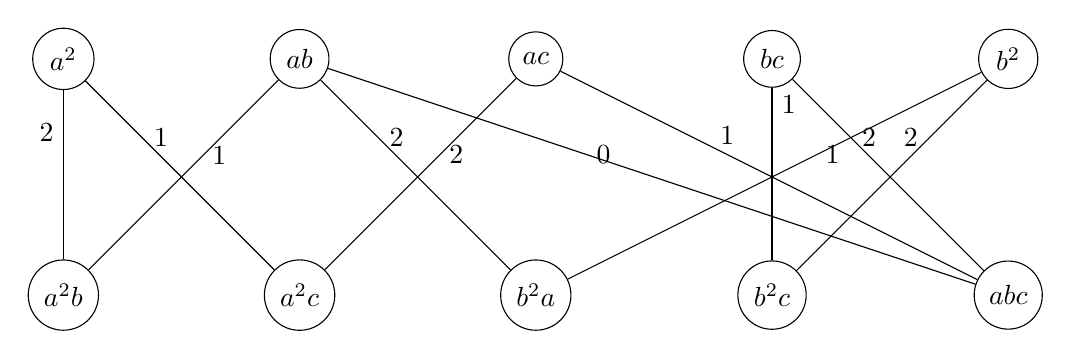
\begin{tikzpicture}[node distance={30mm}, main/.style = {draw, circle}] 
\node[main] (1) {$a^2$}; 
\node[main] (2) [right of=1] {$ab$}; 
\node[main] (3) [right of=2] {$ac$}; 
\node[main] (4) [right of=3] {$bc$}; 
\node[main] (5) [right of=4] {$b^2$}; 

\node[main] (6) [below of=1] {$a^2b$}; 
\node[main] (7) [below of=2] {$a^2c$}; 
\node[main] (8) [below of=3] {$b^2a$}; 
\node[main] (9) [below of=4] {$b^2c$}; 
\node[main] (10) [below of=5] {$abc$}; 

 

\draw (1) -- node[pos=0.25, left] {$2$} (6); 
\draw (1) -- node[pos=0.4, above] {$1$} (7); 

\draw (2) -- node[pos=0.4, right] {$1$}(6); 
\draw (2) -- node[pos=0.4, above] {$2$}(8); 
\draw (2) -- node[pos=0.4, right] {$0$}(10); 


\draw (3) -- node[pos=0.4, right] {$2$}(7); 
\draw (3) -- node[pos=0.4, above] {$1$}(10); 

\draw (4) -- node[pos=0.1, right] {$1$}(9); 
\draw (4) -- node[pos=0.4, above]  {$2$}(10); 

\draw (5) -- node[pos=0.4, right] {$1$}(8); 
\draw (5) -- node[pos=0.4, above] {$2$}(9); 

\end{tikzpicture} 
\end{center}
\caption{граф з вагами, для мультимножини  $ A = \{a^6, b^2, c\} $}
\end{figure}

\section{Частковий випадок $A = \{a^7, b^2, c\}$}

Розглянемо наступний випадок мультимножини виду $A = \{a^7, b^2, c\}$, яка задовольняє умови {\bf Теореми 1}. На елементи накладаються деякі обмеження, а саме потужність усіх елементів рівна, а один єдиний елемент має потужність одиниця.

\begin{example}

Розглянемо множину $ A = \{a^7, b^2, c\} $, збудуємо наповнення 2-елементного сімейства невключних одна в одну множин, які добудуємо до 3-елементного сімейства:
\begin{figure}
\begin{center}
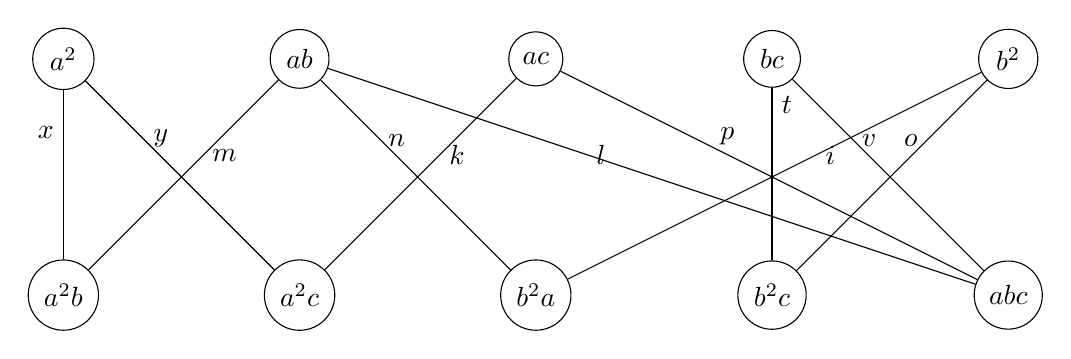
\begin{tikzpicture}[node distance={30mm}, main/.style = {draw, circle}] 
\node[main] (1) {$a^2$}; 
\node[main] (2) [right of=1] {$ab$}; 
\node[main] (3) [right of=2] {$ac$}; 
\node[main] (4) [right of=3] {$bc$}; 
\node[main] (5) [right of=4] {$b^2$}; 

\node[main] (6) [below of=1] {$a^2b$}; 
\node[main] (7) [below of=2] {$a^2c$}; 
\node[main] (8) [below of=3] {$b^2a$}; 
\node[main] (9) [below of=4] {$b^2c$}; 
\node[main] (10) [below of=5] {$abc$}; 

 

\draw (1) -- node[pos=0.25, left] {$x$} (6); 
\draw (1) -- node[pos=0.4, above] {$y$} (7); 

\draw (2) -- node[pos=0.4, right] {$m$}(6); 
\draw (2) -- node[pos=0.4, above] {$n$}(8); 
\draw (2) -- node[pos=0.4, right] {$l$}(10); 


\draw (3) -- node[pos=0.4, right] {$k$}(7); 
\draw (3) -- node[pos=0.4, above] {$p$}(10); 

\draw (4) -- node[pos=0.1, right] {$t$}(9); 
\draw (4) -- node[pos=0.4, above]  {$v$}(10); 

\draw (5) -- node[pos=0.4, right] {$i$}(8); 
\draw (5) -- node[pos=0.4, above] {$o$}(9); 

\end{tikzpicture} 
\end{center}
\caption{граф з вагами, для мультимножини  $ A = \{a^7, b^2, c\} $}
\end{figure}
\end{example}

Так само, як і у випадках раніше підрахуємо значення вагів за формулою:
\begin{center}
$ \underline{deg} = 3 $ - оскільки $ |\{a^2,b\}| = |\{a^2,c\}| = |\{a,b,c\}| = ... $
\\
$ \overline{deg} = |A| - 2 = 3 $, $ |A| = 5, |\{a^2\}| = |\{a,b\}| = |\{b,c\}| =  |\{a,c\}| = ... = 2 $
\end{center}
Нижче записана система лінійних рівнянь та її розв'язок. Як можна побачити усі коефіцієнти невід'ємні та задовольняють умови {\bf Теореми 1}.
\begin{center}
$\left \{
\begin{tabular}{ccc}
x + y = 3 \\
x + m = 3 \\ 
k + y = 3 \\
m + n + l = 3 \\
p + k = 3 \\
n + i = 3 \\
t + v = 3 \\ 
t + b = 3 \\
p + l + v = 3 \\ 
i + l = 3 \\
t + o = 3 \\
  \end{tabular}
\Rightarrow 
$
$\left \{
\begin{tabular}{ccc}
x = 2 \\
y = 1 \\
m = 1 \\ 
p = 1 \\
n = 2 \\
k = 2 \\
v = 2 \\ 
t = 1 \\
l = 0 \\ 
i = 1 \\
o = 2 \\
  \end{tabular}
$
\end{center}

Отже отримали зважений граф при переході від двоелементних мультипідмножин до триелементних мультипідмножин:
\begin{figure}
\begin{center}
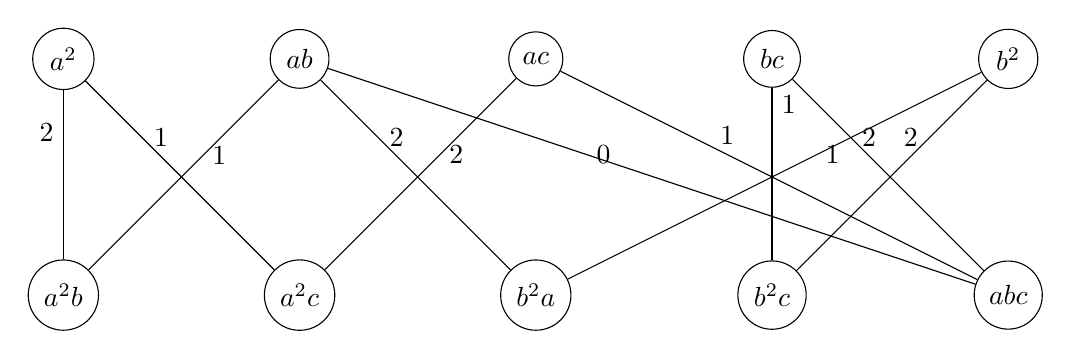
\begin{tikzpicture}[node distance={30mm}, main/.style = {draw, circle}] 
\node[main] (1) {$a^2$}; 
\node[main] (2) [right of=1] {$ab$}; 
\node[main] (3) [right of=2] {$ac$}; 
\node[main] (4) [right of=3] {$bc$}; 
\node[main] (5) [right of=4] {$b^2$}; 

\node[main] (6) [below of=1] {$a^2b$}; 
\node[main] (7) [below of=2] {$a^2c$}; 
\node[main] (8) [below of=3] {$b^2a$}; 
\node[main] (9) [below of=4] {$b^2c$}; 
\node[main] (10) [below of=5] {$abc$}; 

 

\draw (1) -- node[pos=0.25, left] {$2$} (6); 
\draw (1) -- node[pos=0.4, above] {$1$} (7); 

\draw (2) -- node[pos=0.4, right] {$1$}(6); 
\draw (2) -- node[pos=0.4, above] {$2$}(8); 
\draw (2) -- node[pos=0.4, right] {$0$}(10); 


\draw (3) -- node[pos=0.4, right] {$2$}(7); 
\draw (3) -- node[pos=0.4, above] {$1$}(10); 

\draw (4) -- node[pos=0.1, right] {$1$}(9); 
\draw (4) -- node[pos=0.4, above]  {$2$}(10); 

\draw (5) -- node[pos=0.4, right] {$1$}(8); 
\draw (5) -- node[pos=0.4, above] {$2$}(9); 

\end{tikzpicture} 
\end{center}
\caption{граф з вагами, для мультимножини  $ A = \{a^7, b^2, c\} $}
\end{figure}


\section{Частковий випадок $A = \{a^8, b^2, c\}$}

Розглянемо наступний випадок мультимножини виду $A = \{a^8, b^2, c\}$, яка задовольняє умови {\bf Теореми 1}. На елементи накладаються деякі обмеження, а саме потужність усіх елементів рівна, а один єдиний елемент має потужність одиниця.

\begin{example}

Розглянемо множину $ A = \{a^8, b^2, c\} $, збудуємо наповнення двоелементного сімейства невключних одна в одну множин, які добудуємо до триелементного сімейства:
\begin{figure}
\begin{center}
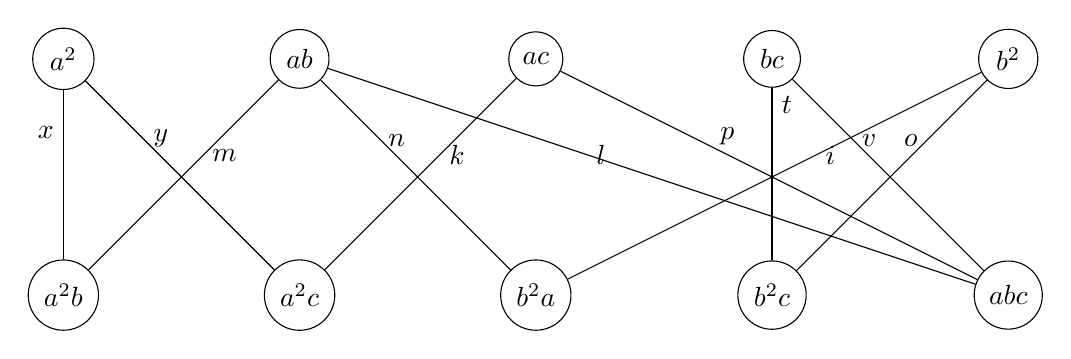
\begin{tikzpicture}[node distance={30mm}, main/.style = {draw, circle}] 
\node[main] (1) {$a^2$}; 
\node[main] (2) [right of=1] {$ab$}; 
\node[main] (3) [right of=2] {$ac$}; 
\node[main] (4) [right of=3] {$bc$}; 
\node[main] (5) [right of=4] {$b^2$}; 

\node[main] (6) [below of=1] {$a^2b$}; 
\node[main] (7) [below of=2] {$a^2c$}; 
\node[main] (8) [below of=3] {$b^2a$}; 
\node[main] (9) [below of=4] {$b^2c$}; 
\node[main] (10) [below of=5] {$abc$}; 

 

\draw (1) -- node[pos=0.25, left] {$x$} (6); 
\draw (1) -- node[pos=0.4, above] {$y$} (7); 

\draw (2) -- node[pos=0.4, right] {$m$}(6); 
\draw (2) -- node[pos=0.4, above] {$n$}(8); 
\draw (2) -- node[pos=0.4, right] {$l$}(10); 


\draw (3) -- node[pos=0.4, right] {$k$}(7); 
\draw (3) -- node[pos=0.4, above] {$p$}(10); 

\draw (4) -- node[pos=0.1, right] {$t$}(9); 
\draw (4) -- node[pos=0.4, above]  {$v$}(10); 

\draw (5) -- node[pos=0.4, right] {$i$}(8); 
\draw (5) -- node[pos=0.4, above] {$o$}(9); 

\end{tikzpicture} 
\end{center}
\caption{граф з вагами, для мультимножини  $ A = \{a^8, b^2, c\} $}
\end{figure}
\end{example}

Так само, як і у випадках раніше підрахуємо значення вагів за формулою:
\begin{center}
$ \underline{deg} = 3 $ - оскільки $ |\{a^2,b\}| = |\{a^2,c\}| = |\{a,b,c\}| = ... $
\\
$ \overline{deg} = |A| - 2 = 3 $, $ |A| = 5, |\{a^2\}| = |\{a,b\}| = |\{b,c\}| =  |\{a,c\}| = ... = 2 $
\end{center}
Нижче записана система лінійних рівнянь та її розв'язок. Як можна побачити усі коефіцієнти невід'ємні та задовольняють умови {\bf Теореми 1}.
\begin{center}
$\left \{
\begin{tabular}{ccc}
x + y = 3 \\
x + m = 3 \\ 
k + y = 3 \\
m + n + l = 3 \\
p + k = 3 \\
n + i = 3 \\
t + v = 3 \\ 
t + b = 3 \\
p + l + v = 3 \\ 
i + l = 3 \\
t + o = 3 \\
  \end{tabular}
\Rightarrow 
$
$\left \{
\begin{tabular}{ccc}
x = 2 \\
y = 1 \\
m = 1 \\ 
p = 1 \\
n = 2 \\
k = 2 \\
v = 2 \\ 
t = 1 \\
l = 0 \\ 
i = 1 \\
o = 2 \\
  \end{tabular}
$
\end{center}

Отже отримали зважений граф при переході від двоелементних мультипідмножин до триелементних мультипідмножин:
\begin{figure}
\begin{center}
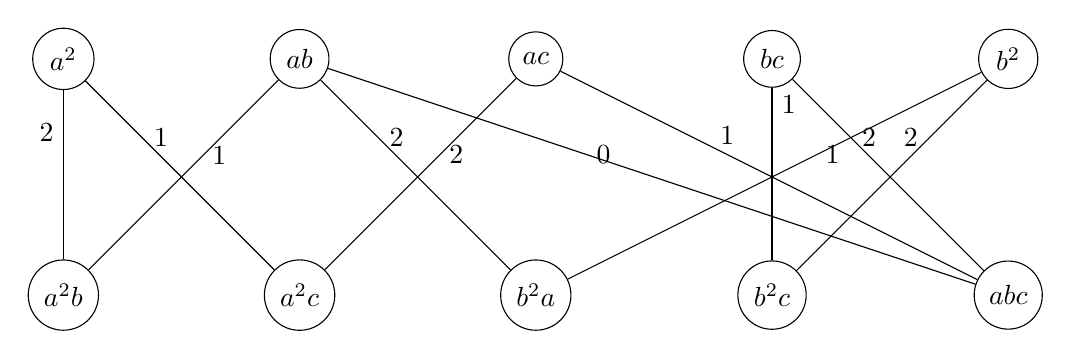
\begin{tikzpicture}[node distance={30mm}, main/.style = {draw, circle}] 
\node[main] (1) {$a^2$}; 
\node[main] (2) [right of=1] {$ab$}; 
\node[main] (3) [right of=2] {$ac$}; 
\node[main] (4) [right of=3] {$bc$}; 
\node[main] (5) [right of=4] {$b^2$}; 

\node[main] (6) [below of=1] {$a^2b$}; 
\node[main] (7) [below of=2] {$a^2c$}; 
\node[main] (8) [below of=3] {$b^2a$}; 
\node[main] (9) [below of=4] {$b^2c$}; 
\node[main] (10) [below of=5] {$abc$}; 

 

\draw (1) -- node[pos=0.25, left] {$2$} (6); 
\draw (1) -- node[pos=0.4, above] {$1$} (7); 

\draw (2) -- node[pos=0.4, right] {$1$}(6); 
\draw (2) -- node[pos=0.4, above] {$2$}(8); 
\draw (2) -- node[pos=0.4, right] {$0$}(10); 


\draw (3) -- node[pos=0.4, right] {$2$}(7); 
\draw (3) -- node[pos=0.4, above] {$1$}(10); 

\draw (4) -- node[pos=0.1, right] {$1$}(9); 
\draw (4) -- node[pos=0.4, above]  {$2$}(10); 

\draw (5) -- node[pos=0.4, right] {$1$}(8); 
\draw (5) -- node[pos=0.4, above] {$2$}(9); 

\end{tikzpicture} 
\end{center}
\caption{граф з вагами, для мультимножини  $ A = \{a^8, b^2, c\} $}
\end{figure}


\section{Частковий випадок $A = \{a^9, b^2, c\}$}

Розглянемо наступний випадок мультимножини виду $A = \{a^9, b^2, c\}$, яка задовольняє умови {\bf Теореми 1}. На елементи накладаються деякі обмеження, а саме потужність усіх елементів рівна, а один єдиний елемент має потужність одиниця. Зупинимось на ітерації для якої множина  $A = \{a^n, b^2, c\}$, приймає вигляд $A = \{a^9, b^2, c\}$, тобто $n = 9$. Також дуже важливо зазначити, що отримані математичні об'єкти можна використовувати у задачі сильних та слабких груп, яка буде розглянута у розділі практичних застосувань.

\begin{example}

Розглянемо множину $ A = \{a^9, b^2, c\} $, збудуємо наповнення двоелементного сімейства невключних одна в одну множин, які добудуємо до триелементного сімейства:
\begin{figure}
\begin{center}
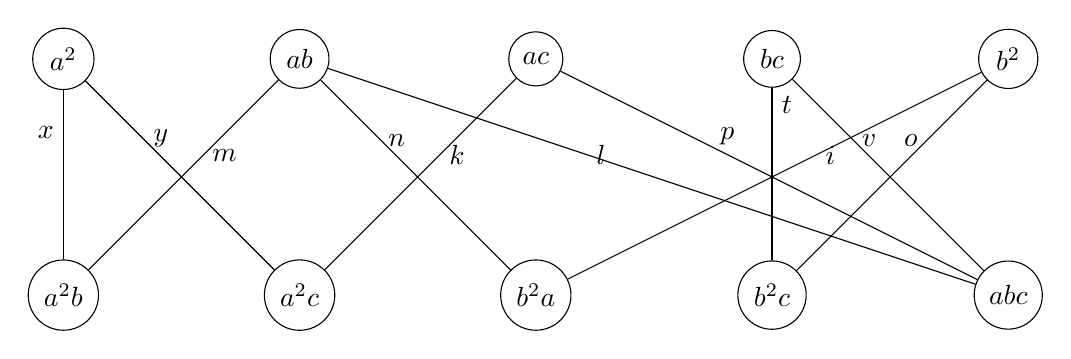
\begin{tikzpicture}[node distance={30mm}, main/.style = {draw, circle}] 
\node[main] (1) {$a^2$}; 
\node[main] (2) [right of=1] {$ab$}; 
\node[main] (3) [right of=2] {$ac$}; 
\node[main] (4) [right of=3] {$bc$}; 
\node[main] (5) [right of=4] {$b^2$}; 

\node[main] (6) [below of=1] {$a^2b$}; 
\node[main] (7) [below of=2] {$a^2c$}; 
\node[main] (8) [below of=3] {$b^2a$}; 
\node[main] (9) [below of=4] {$b^2c$}; 
\node[main] (10) [below of=5] {$abc$}; 

 

\draw (1) -- node[pos=0.25, left] {$x$} (6); 
\draw (1) -- node[pos=0.4, above] {$y$} (7); 

\draw (2) -- node[pos=0.4, right] {$m$}(6); 
\draw (2) -- node[pos=0.4, above] {$n$}(8); 
\draw (2) -- node[pos=0.4, right] {$l$}(10); 


\draw (3) -- node[pos=0.4, right] {$k$}(7); 
\draw (3) -- node[pos=0.4, above] {$p$}(10); 

\draw (4) -- node[pos=0.1, right] {$t$}(9); 
\draw (4) -- node[pos=0.4, above]  {$v$}(10); 

\draw (5) -- node[pos=0.4, right] {$i$}(8); 
\draw (5) -- node[pos=0.4, above] {$o$}(9); 

\end{tikzpicture} 
\end{center}
\caption{граф з вагами, для мультимножини  $ A = \{a^9, b^2, c\} $}
\end{figure}
\end{example}

Так само, як і у випадках раніше підрахуємо значення вагів за формулою:
\begin{center}
$ \underline{deg} = 3 $ - оскільки $ |\{a^2,b\}| = |\{a^2,c\}| = |\{a,b,c\}| = ... $
\\
$ \overline{deg} = |A| - 2 = 3 $, $ |A| = 5, |\{a^2\}| = |\{a,b\}| = |\{b,c\}| =  |\{a,c\}| = ... = 2 $
\end{center}
Нижче записана система лінійних рівнянь та її розв'язок. Як можна побачити усі коефіцієнти невід'ємні та задовольняють умови {\bf Теореми 1}.
\begin{center}
$\left \{
\begin{tabular}{ccc}
x + y = 3 \\
x + m = 3 \\ 
k + y = 3 \\
m + n + l = 3 \\
p + k = 3 \\
n + i = 3 \\
t + v = 3 \\ 
t + b = 3 \\
p + l + v = 3 \\ 
i + l = 3 \\
t + o = 3 \\
  \end{tabular}
\Rightarrow 
$
$\left \{
\begin{tabular}{ccc}
x = 2 \\
y = 1 \\
m = 1 \\ 
p = 1 \\
n = 2 \\
k = 2 \\
v = 2 \\ 
t = 1 \\
l = 0 \\ 
i = 1 \\
o = 2 \\
  \end{tabular}
$
\end{center}

Отже отримали зважений граф при переході від двоелементних мультипідмножин до триелементних мультипідмножин:
\begin{figure}
\begin{center}
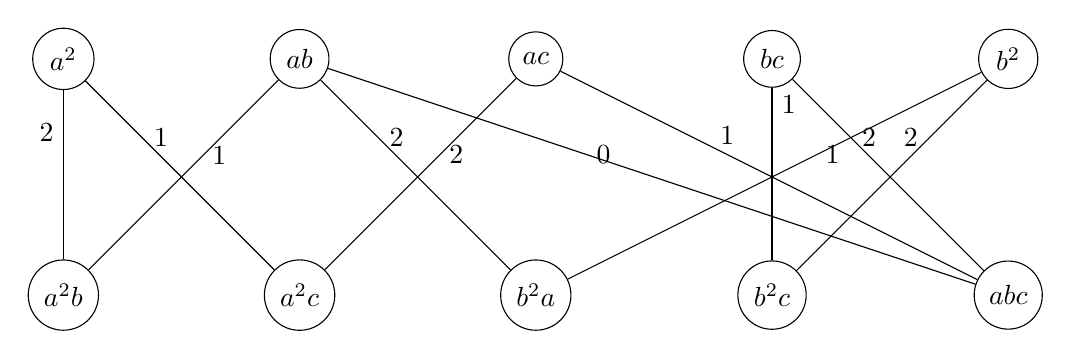
\begin{tikzpicture}[node distance={30mm}, main/.style = {draw, circle}] 
\node[main] (1) {$a^2$}; 
\node[main] (2) [right of=1] {$ab$}; 
\node[main] (3) [right of=2] {$ac$}; 
\node[main] (4) [right of=3] {$bc$}; 
\node[main] (5) [right of=4] {$b^2$}; 

\node[main] (6) [below of=1] {$a^2b$}; 
\node[main] (7) [below of=2] {$a^2c$}; 
\node[main] (8) [below of=3] {$b^2a$}; 
\node[main] (9) [below of=4] {$b^2c$}; 
\node[main] (10) [below of=5] {$abc$}; 

 

\draw (1) -- node[pos=0.25, left] {$2$} (6); 
\draw (1) -- node[pos=0.4, above] {$1$} (7); 

\draw (2) -- node[pos=0.4, right] {$1$}(6); 
\draw (2) -- node[pos=0.4, above] {$2$}(8); 
\draw (2) -- node[pos=0.4, right] {$0$}(10); 


\draw (3) -- node[pos=0.4, right] {$2$}(7); 
\draw (3) -- node[pos=0.4, above] {$1$}(10); 

\draw (4) -- node[pos=0.1, right] {$1$}(9); 
\draw (4) -- node[pos=0.4, above]  {$2$}(10); 

\draw (5) -- node[pos=0.4, right] {$1$}(8); 
\draw (5) -- node[pos=0.4, above] {$2$}(9); 

\end{tikzpicture} 
\end{center}
\caption{граф з вагами, для мультимножини  $ A = \{a^9, b^2, c\} $}
\end{figure}


\section{Статистичний аналіз розміру антиланцюга}

Нехай дана мультимножина $M = \{a_1^{m_1}, ... , a_n^{m_n}\} $. Підрахуємо кількість усіх можливих підмножин зі зваженою потужністю $k$:
\begin{center}
$ 0 \leq k \leq |M|= m_1 + ... + m_n$
\end{center}

Тоді будь-якій підмножині $ L \subseteq  M $ виду $\{a_1^{x_1}, ... , a_n^{x_n}\} $ ставимо у відповідність вектор:

\begin{center}
$ \overrightarrow{x} = (x_1, ..., x_n) $, де $0 \leq x_1 \leq m1, ..., 0 \leq x_n \leq m_n$.
\end{center}

Треба розв'язати підзадачу і знайти кількість векторів $ \overrightarrow{x} = (x_1, ..., x_n) $, які задовольняють умовам ($l$ - деяке число таке, що $0 \leq l \leq n$):


\begin{center}
$\left \{
\begin{tabular}{ccc}
x_1 + ... + x_n = k  \\
0 \leq x_1 \leq m1, ..., 0 \leq x_l \leq m_l \\ 
x_{l+1} = ... = x_n = 0 \\
\end{tabular}
$
\end{center}

Нехай $D_l^k$ - відповідь на підзадачу для заданих $l$ та $k$, тоді очевидно, що:

\begin{center}
$D_0^k = 1$, якщо $k=0$
\\
$D_0^k = 0$, якщо $k \neq 0$
\end{center}

Також очевидно, що:
\begin{center}
$D_{l+1}^k = D_l^k + D_l^{k-1} + ... + D_l^{k-m_{l+1}}$
\end{center}

У формулі наведеній вижче кожен доданок виду $D_l^{k-l}$ ставиться у відповідність підмножинам, в яких кратність елемента $a_{l+1}$ дорівнює $b$ ($0 \leq b \leq m_{l+1} $).
Розглянемо простий випадок:
\begin{center}
$k \leq m_1,..., k \leq  m_n$
\end{center}
Тоді на вектор  $ \overrightarrow{x} = (x_1, ..., x_n) $ накладається лише одна умова:

\begin{center}
$x_1 + ... + x_n = k $, $x_1,...,x_n \in \mathbb {N} \cup \{0\}$
\end{center}

Перепишемо цю умову додавшидо кожного $x_i$ одиницю з лівої частини, та додавши $n$ з правої:
\begin{center}
$(x_1 + 1) ... + (x_n + 1) = k + n $
\\
$x_1,...,x_n \in \mathbb {N} \cup \{0\}$
\end{center}

А тепер перепишемо цю формулу зважаючи на нові позначення:
\begin{center}
$y_1 + ... + y_n = k + n$
\\
$y_1 = x_1 + 1, ..., y_n = x_n + 1$
\\
$y_1,...,y_n \in \mathbb {N}$
\end{center}

Представимо розбиття числа $k+n$ у суму $y_1 + ... + y_n$, як розріз полоски розміром $1 \times (k+n)$ на полоски розмірами $1 \times y_1,...,1 \times y_n$:

\begin{example}
Розглянемо рівняння $ y_1 + y_2 + y_3 = 5 $:
\begin{center}
$ 5 = 3 + 1 + 1 $
\\
$ 5 = 2 + 2 + 1 $
\\
$ 5 = 2 + 1 + 2 $
\\
$ 5 = 1 + 3 + 1 $
\\
$ 5 = 1 + 2 + 2 $
\\
$ 5 = 1 + 1 + 3 $
\end{center}
\end{example}

Кожен переріз - це вибір $(n-1)$ розрізу з$(k+n-1)$ можливих, тобто:
\begin{center}
$C_{k+n-1}^{n-1}$
\end{center}

Як довести, що $D_n^{[|M|/2]}$ - найбільша (нестрого) з усіх $D_n^x (0 \leq x \leq |M|)$? Використовуючи індукцію по $n$ доведемо, що:
\begin{center}
$ D_n^0 \leq D_n^1 \leq ... \leq D_n^{[|M|/2]}$.
\end{center}
Очевидний факт, що $D_n^x = D_n^{|M|-x}$ - інверсія множини.

\begin{proof}
Якщо $k \leq [|M|/2]$, то $D_n^k \leq D_n^{k+1}$:
\begin{center}
$k = (n-1)/2$, тоді $D_n^k \leq D_n^{k+1}$
\\
$k \leq n/2 - 1$, тоді $D_n^k = D_{n-1}^k D_{n-1}^{k-1}$
\end{center}
Використаємо нерівність:
\begin{center}
$D_{n-1}^k + D_{n-1}^{k-1} \leq D_{n-1}^{k+1} + D_{n-1}^{k}$
\end{center}
Скоротивши отримаємо:
\begin{center}
$D_{n-1}^{k-1} \leq D_{n-1}^{k+1}$
\end{center}

Твердження індукції:
\begin{center}
$ D_n^0 \leq D_n^1 \leq ... \leq D_n^{[|M|/2]}$
\end{center}

Оскільки $k \leq n/2 - 1$, то $k \leq (n - 2)/2$, тоді $k < (n - 1)/2$.
\begin{center}
$D_{n-1}^{k} \leq D_{n-1}^{k-1}$
\\
$D_{n-1}^{k} < D_{n-1}^{k-1}$
\end{center}

Задекларуємо мультимножини:

\begin{center}
$M = \{a_1^{x_1}, ... , a_n^{x_n}\} $ 
\\
$\overline{M} = \{a_1^{x_1}, ... , a_{n-1}^{x_{n-1}}\} $ 
\end{center}

Нехай $D_{|M|}^k $ кількість $k$ елементних мультивибірок з $M$, тоді  $D_{|M|}^k =  D_{\overline{|M|}}^k + D_{\overline{|M|}}
^{k-1} + ... + D_{\overline{|M|}}^{k-x} = 0  $, враховуючи, що $D_{|M|}^k  = D_{|M|}^{\overline{|M|} - k}$. 
\\
Доведення по індукції: $D_{|M|}^k  = D_{\overline{|M|}}^{k-b_n} + ... + D_{\overline{|M|}}^k$, де $\overline{M} = D \setminus {a_n^{b_n}}$.

\end{proof}

Для підрахунку більш складних випадків, коли кількість елементів у мультимножині довільна та потужність кожного елемента теж довільна, можна використати формулу включень та виключень задля вирішення задачі, тобто обрахунок для кожного елемента ведеться для тих мультипідмножин яким він належить та з яких виключається, щоб виключити повтори:
\begin{center}
${\displaystyle \left|\bigcup _{i=1}^{n}A_{i}\right|=\sum _{k=1}^{n}(-1)^{k+1}\left(\sum _{1\leqslant i_{1}<\cdots <i_{k}\leqslant n}|A_{i_{1}}\cap \cdots \cap A_{i_{k}}|\right)}$
\end{center}


\section*{Висновки до розділу 2}
\addcontentsline{toc}{chapter}{Висновки до розділу 2}

	Розглянуто та доведено частинні випадки, які задовольняють умови теореми. Розглянуто та запропоновано можливість статистичного обрахунку потужності сімейства невкладених одна в одну мультипідмножин. Запропоновано нові можливості доведення ускладнених випадків теореми та розширено частинні випадки, які можна використовувати для прикладних задач.
\newpage

\chapter{Практичне застосування}

\section{Теорія голосування}
Система голосування на множині виду $M = \{a_1^{x_1}, ... , a_n^{x_n}\}$ - це така функція:

\begin{center}
$F = B(M) \rightarrow \{0,1\}$
\\
$ \forall A, B \subseteq M: A \subseteq B$, то $F(A) \leq F(B)$ 
\\
Де $B(M)$ - сімейство всіх мультипідмножин $L \subseteq M$
\end{center}

Звернемо увагу, що $F$ взаємно-однозначно задається набором "мінімальних прохідних підмножин":

\begin{center}
$F(L) = 1, L \subseteq M $
\\
$ \forall K \subset L: F(K) = 0$ 
\end{center}

Сімейство невкладених одна в одну множин \cite{my_article:2021} має дуже важливе значення, оскільки представляє собою набір множин які неможливо порівняти між собою у рамках задачі теорії голосувань. Можливість мати на примітку множини, які задовольняють умови {\bf Теореми 1} є дуже важливим прикладним моментом, оскільки в теорїї голосувань ми будемо мати безпосередньо мати справу з цими множинами, а отже мати представлення про потужність та структуру таких множин є дуже важливим прикладним нюансом.

Множина $M = \{a_1^{x_1}, ... , a_n^{x_n}\}$ може представляти партії, а кожен елемент $a_i$ - одиницю партії, тобто людину, яка може віддати свій голос. Кожна людина яка належить одній партії буде розлянута, як еквівалентна в рамках даної партії, тобто голоси таких виборчих одиниць є рівнозначними. Підсумуємо: множина $M = \{a_1^{x_1}, ... , a_n^{x_n}\}$, складається з партій $a_i$, а $x_i$ - це кількість виборчих одиниць у партії (людей).


\section{Потоки у графах}

У теорії алгоритмів та дослідженні операцій проблема максимального потоку включають пошук можливого потоку на графі через мережу потоків. Ця задача має дуже важливе значення, оскільки проблеми, які вирішуються за допомогою урівноваження графу, та пошуку найкоротшого та найдешевшого шляху дуже важливі у транспортних задачах.

Проблему максимального потоку можна розглядати як окремий випадок більш складних проблем, таких як проблема циркуляції. Максимальне значення потоку дорівнює мінімальній пропускній здатності розрізу у мережі, як зазначено в мінімальному максимальному потоку. З точки зору задачі, яка розгядається у даній роботі, ми розглянемо частковий випадок транспортної задачі, де роль пунктів  заїзду (доставки) товарів відіграють долі двочасткового графу. Задача є виокремленою чатиною та є підмножиною загальних транспортих задач.

Розглянемо застосування даного способу балансування графу на прикладі:

\begin{figure}[!htb]
\begin{center}
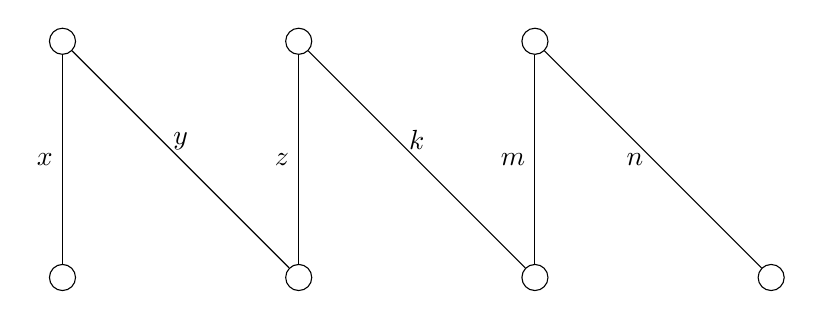
\begin{tikzpicture}[node distance={30mm}, main/.style = {draw, circle}] 
\node[main] (1) {$  $}; 
\node[main] (2) [right of=1] {$  $}; 
\node[main] (3) [right of=2] {$  $}; 
\node[main] (4) [below of=1] {$  $}; 
\node[main] (5) [below of=2] {$  $};
\node[main] (6) [below of=3] {$  $}; 
\node[main] (7) [right of=6] {$  $}; 

\draw (1) -- node[left]  {$x$} (4); 
\draw (1) -- node[above] {$y$} (5); 
\draw (2) -- node[left]  {$z$} (5); 
\draw (2) -- node[above] {$k$} (6); 
\draw (3) -- node[left]  {$m$} (6); 
\draw (3) -- node[left]  {$n$} (7); 
\end{tikzpicture} 
\end{center}
\caption{приклад системи для балансування}
\end{figure}

З моєї бакалаврської роботи відомо випадок, який було доведено, а саме $K=\{a^m,b^n\}$, тобто елемент $a$ має потужність $m$, а елемент $b$ --- $n$. Для цього випадку було отримано явний вид формул, за допомогою яких можна увантахити граф. 

Тобто для системи, яка може бути представлена у вигляді двочасткового графу, де кожна доля представляє собою однотипні рівноважні вузли, іншими словами всі вузли, які належать одній долі графу - еквівалентні та мають одну вагу. Для прикладу це можуть бути джерелами споживання напруги, а ребра - це проводи з відповідними коефіцієнтами опору (дуже грубий приклад). Тоді можна відповідно вирішивши систему рівнянь, перед цим задавши ступені для верхньої та нижньої долі, отримати навантаження для кожногоребра задля балансування графу. Отже, якщо взяти за приклад мультимножину, для якох вже було доведено ускладнений випадок теореми, та обрахувати ступені вхождення для кожної долі, можна отримати зважену систему. Тож розглянемо приклад:

Нехай $K = \{2,2,2,3,3\}$, тобто множина $ K \subseteq \{a^m,b^n\}$.

\begin{figure}[!htb]
\begin{center}
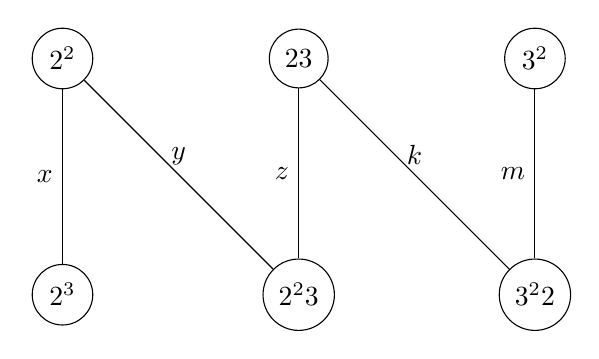
\begin{tikzpicture}[node distance={30mm}, main/.style = {draw, circle}] 
\node[main] (1) {$2^2$}; 
\node[main] (2) [right of=1] {$2 3$}; 
\node[main] (3) [right of=2] {$3^2$}; 
\node[main] (4) [below of=1] {$2^3$}; 
\node[main] (5) [below of=2] {$2^2 3$};
\node[main] (6) [below of=3] {$3^2 2$}; 

\draw (1) -- node[left]  {$x$} (4); 
\draw (1) -- node[above] {$y$} (5); 
\draw (2) -- node[left]  {$z$} (5); 
\draw (2) -- node[above] {$k$} (6); 
\draw (3) -- node[left]  {$m$} (6); 
\end{tikzpicture} 
\end{center}
\caption{приклад системи для балансування}
\end{figure}

Так само, як і у випадках раніше підрахуємо значення вагів за формулою:
\begin{center}
$ \underline{deg} = 3 $ - оскільки $ |\{2^2\}| = |\{2,3\}| = |\{3^2\}| = 3 $
\\
$ \overline{deg} = |K| - 2 = 3 $, $ |K| = 5, |\{3^2,2\}| = |\{2^2,3\}| = |\{b,c\}| =  |\{2^3\}| = 3 $
\end{center}

Як можна бачити отримали $ \underline{deg} = \overline{deg} = 3 $, задля зручності можна розілити отримані коефіцієнти на $3$, тобто потужності ступенів входу у верхню та нижню долі дорівнюють одиниці.

\begin{center}
$\left \{
\begin{tabular}{ccc}
x + y = 1  \\
y + z = 1 \\ 
z + k = 1 \\ 
k + m = 1 \\ 
\end{tabular}
$
\end{center}

\begin{center}
$\left \{
\begin{tabular}{ccc}
x = 1  \\
y = 0 \\ 
z = 1 \\ 
k = 0 \\
m = 1 \\ 
\end{tabular}
$
\end{center}


Нехай $K = \{2,2,2,3,3,3\}$, тобто множина $ K \subseteq \{a^m,b^n\}$.

\begin{figure}[!htb]
\begin{center}
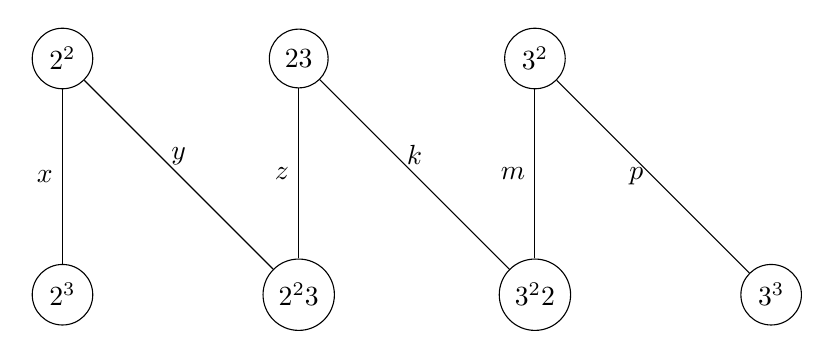
\begin{tikzpicture}[node distance={30mm}, main/.style = {draw, circle}] 
\node[main] (1) {$2^2$}; 
\node[main] (2) [right of=1] {$2 3$}; 
\node[main] (3) [right of=2] {$3^2$}; 
\node[main] (4) [below of=1] {$2^3$}; 
\node[main] (5) [below of=2] {$2^2 3$};
\node[main] (6) [below of=3] {$3^2 2$}; 
\node[main] (7) [right of=6] {$3^3$}; 


\draw (1) -- node[left]  {$x$} (4); 
\draw (1) -- node[above] {$y$} (5); 
\draw (2) -- node[left]  {$z$} (5); 
\draw (2) -- node[above] {$k$} (6); 
\draw (3) -- node[left]  {$m$} (6); 
\draw (3) -- node[left]  {$p$} (7); 

\end{tikzpicture} 
\end{center}
\caption{приклад системи для балансування}
\end{figure}

Так само, як і у випадках раніше підрахуємо значення вагів за формулою:
\begin{center}
$ \underline{deg} = 3 $ - оскільки $ |\{2^2\}| = |\{2,3\}| = |\{3^2,2\}| = 3 $
\\
$ \overline{deg} = |K| - 2 = 4 $, $ |K| = 6, |\{3^2,2\}| = |\{2^2,3\}| = |\{b,c\}| =  |\{2^3\}| = 3 $
\end{center}

Як можна бачити отримали $ \underline{deg}  = 3, \overline{deg} = 4 $, задля зручності можна розілити отримані коефіцієнти на $3$, тобто потужності ступенів входу у верхню та нижню долі дорівнюють одиниці.

\begin{center}
$\left \{
\begin{tabular}{ccc}
x + y = 4  \\
y + z = 3 \\ 
z + k = 4 \\ 
k + m = 3 \\ 
m + p = 4 \\ 
p = 3 \\
\end{tabular}
$
\end{center}

\begin{center}
$\left \{
\begin{tabular}{ccc}
x = 3  \\
y = 1 \\ 
z = 2 \\ 
k = 2 \\
m = 1 \\ 
p = 3 \\
\end{tabular}
$
\end{center}

Таким же чином можна застосувати даний тип увантаження на часткових випадках, які були доведені вище, наприклад:

Для системи, яка має вигляд, або описується множиною  $ A = \{a^9, b^2, c\} $, задано граф, який явно можна увантажити:

\begin{figure}
\begin{center}
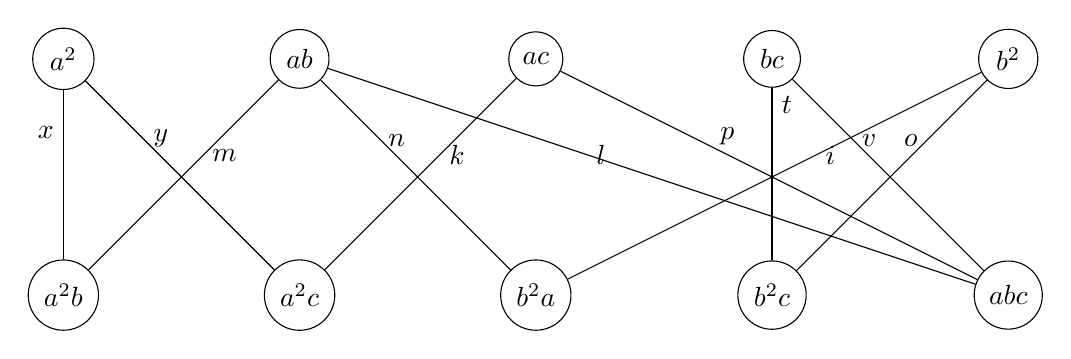
\begin{tikzpicture}[node distance={30mm}, main/.style = {draw, circle}] 
\node[main] (1) {$a^2$}; 
\node[main] (2) [right of=1] {$ab$}; 
\node[main] (3) [right of=2] {$ac$}; 
\node[main] (4) [right of=3] {$bc$}; 
\node[main] (5) [right of=4] {$b^2$}; 

\node[main] (6) [below of=1] {$a^2b$}; 
\node[main] (7) [below of=2] {$a^2c$}; 
\node[main] (8) [below of=3] {$b^2a$}; 
\node[main] (9) [below of=4] {$b^2c$}; 
\node[main] (10) [below of=5] {$abc$}; 

 

\draw (1) -- node[pos=0.25, left] {$x$} (6); 
\draw (1) -- node[pos=0.4, above] {$y$} (7); 

\draw (2) -- node[pos=0.4, right] {$m$}(6); 
\draw (2) -- node[pos=0.4, above] {$n$}(8); 
\draw (2) -- node[pos=0.4, right] {$l$}(10); 


\draw (3) -- node[pos=0.4, right] {$k$}(7); 
\draw (3) -- node[pos=0.4, above] {$p$}(10); 

\draw (4) -- node[pos=0.1, right] {$t$}(9); 
\draw (4) -- node[pos=0.4, above]  {$v$}(10); 

\draw (5) -- node[pos=0.4, right] {$i$}(8); 
\draw (5) -- node[pos=0.4, above] {$o$}(9); 

\end{tikzpicture} 
\end{center}
\caption{граф з вагами, для мультимножини  $ A = \{a^9, b^2, c\} $}
\end{figure}
\end{example}

Так само, як і у випадках раніше підрахуємо значення вагів за формулою:
\begin{center}
$ \underline{deg} = 3 $ - оскільки $ |\{a^2,b\}| = |\{a^2,c\}| = |\{a,b,c\}| = ... $
\\
$ \overline{deg} = |A| - 2 = 3 $, $ |A| = 5, |\{a^2\}| = |\{a,b\}| = |\{b,c\}| =  |\{a,c\}| = ... = 2 $
\end{center}

\begin{center}
$\left \{
\begin{tabular}{ccc}
x + y = 3 \\
x + m = 3 \\ 
k + y = 3 \\
m + n + l = 3 \\
p + k = 3 \\
n + i = 3 \\
t + v = 3 \\ 
t + b = 3 \\
p + l + v = 3 \\ 
i + l = 3 \\
t + o = 3 \\
  \end{tabular}
\Rightarrow 
$
$\left \{
\begin{tabular}{ccc}
x = 2 \\
y = 1 \\
m = 1 \\ 
p = 1 \\
n = 2 \\
k = 2 \\
v = 2 \\ 
t = 1 \\
l = 0 \\ 
i = 1 \\
o = 2 \\
  \end{tabular}
$
\end{center}


\begin{figure}
\begin{center}
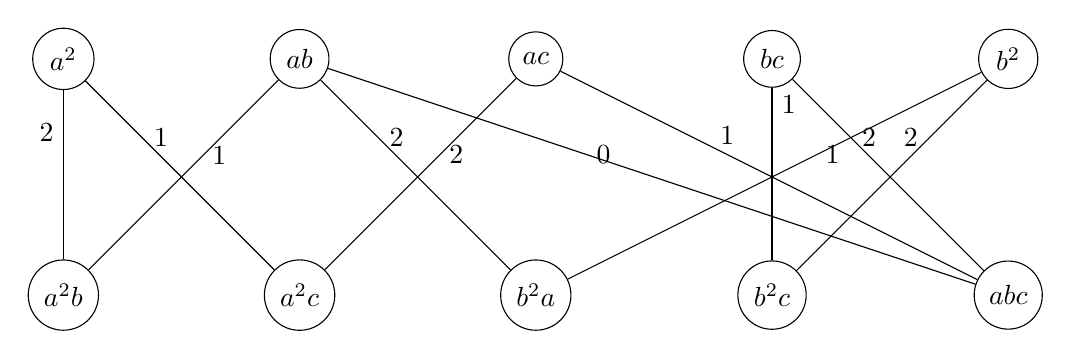
\begin{tikzpicture}[node distance={30mm}, main/.style = {draw, circle}] 
\node[main] (1) {$a^2$}; 
\node[main] (2) [right of=1] {$ab$}; 
\node[main] (3) [right of=2] {$ac$}; 
\node[main] (4) [right of=3] {$bc$}; 
\node[main] (5) [right of=4] {$b^2$}; 

\node[main] (6) [below of=1] {$a^2b$}; 
\node[main] (7) [below of=2] {$a^2c$}; 
\node[main] (8) [below of=3] {$b^2a$}; 
\node[main] (9) [below of=4] {$b^2c$}; 
\node[main] (10) [below of=5] {$abc$}; 

 

\draw (1) -- node[pos=0.25, left] {$2$} (6); 
\draw (1) -- node[pos=0.4, above] {$1$} (7); 

\draw (2) -- node[pos=0.4, right] {$1$}(6); 
\draw (2) -- node[pos=0.4, above] {$2$}(8); 
\draw (2) -- node[pos=0.4, right] {$0$}(10); 


\draw (3) -- node[pos=0.4, right] {$2$}(7); 
\draw (3) -- node[pos=0.4, above] {$1$}(10); 

\draw (4) -- node[pos=0.1, right] {$1$}(9); 
\draw (4) -- node[pos=0.4, above]  {$2$}(10); 

\draw (5) -- node[pos=0.4, right] {$1$}(8); 
\draw (5) -- node[pos=0.4, above] {$2$}(9); 

\end{tikzpicture} 
\end{center}
\caption{граф з вагами, для мультимножини  $ A = \{a^9, b^2, c\} $}
\end{figure}


\section{Сильні та слабкі групи}

Розглянемо  булеан множини $A = \{1,...,n\}$ та позначимо його як $2^A$, тоді цей булеан можна розбити на два класи $X$ та $Y$, причому:

\begin{center}
$X \cup Y = 2^A$
\\
$X \cap Y = \emptyset $
\\
$\forall N \in X \forall M \in Y: N \nsubset M  $     
\end{center}

Розглянемо сімейство $K$ min сильних підмножин, тобто всіх таких $N ∈ X$, що $ Y \nexists N \in X : Y ⊂ X$. Будь-яке розбиття $(X,Y)$ задає набір $K$. Тобто, за допомогою доведення ускладненого випадку теореми, отримано можливість оцінити розмір сімейства $K$.

\section*{Висновки до розділу 3}
\addcontentsline{toc}{chapter}{Висновки до розділу 3}


	Розглянуто прикладні можливості застосування теореми у задачах: "Теорія Голосувань", "Балансування на графі" та "Сильні та Слабкі групи". Приведено приклади застосування теореми для цих задач. Наведено та описано сутність задач та їх важливість у повсякденному світі. Розглянуто застосування доведених частинних випадків для наведених задач.
